\documentclass[a4paper,12pt]{article}
\usepackage[utf8]{inputenc}
\usepackage{graphicx}
\usepackage{amsmath}
\usepackage{color}   %May be necessary if you want to color links
\usepackage{hyperref}
\usepackage{float}
\usepackage{caption}
\usepackage{wrapfig}
\usepackage{todonotes}
\hypersetup{
    colorlinks=true, %set true if you want colored links
    linktoc=all,     %set to all if you want both sections and subsections linked
    linkcolor=blue,  %choose some color if you want links to stand out
}

\hypersetup{
    colorlinks,
    citecolor=black,
    filecolor=black,
    linkcolor=black,
    urlcolor=black
}

\graphicspath{{./fig/sgv/}}

%opening
\title{Work on SGV and Pandora}
\author{E. Brianne, J. List, M. Berggren}
\date{}

\begin{document}

\maketitle

\begin{abstract}

This paper is done in order to keep track of the work I have done on SGV and the Particle Flow parametrization. This paper will be divided in several parts : Particle Flow in full simulation and SGV, and my Particle Flow studies (Double-counted and lost energy, Energy fraction, Energy density and nearest neighbour). Some of the checks done are then used for benchmarking the performance of the particle flow parametrization in SGV compared to the full simulation.

The main idea found after all this, is the question of how to model the behaviour of Pandora when the \textbf{energy density }is high, typically in high energetic jets. More discrepancies between the current version of SGV and full simulation appear for these high energetic jets (over 100 GeV). In such cases, Pandora is switching to an Energy flow mode. 

The idea is then to parametrize this behaviour in SGV mostly for high energetic jets by certainly changing the distributions that SGV use to parametrise the particle flow (the idea is to take into account in theses distributions, the energy density around a cluster - high density means more chance of splitting off the charge cluster to a neutral cluster).

\end{abstract}

\cleardoublepage
\tableofcontents
\cleardoublepage

\section{Introduction}

First of all, what is Particle Flow? Particle Flow is a new approach to calorimetry in order to achieve a jet energy resolution much better than traditional calorimetry approaches (order of twice better). It has a potential to revolutionise particle detector design for future lepton collider experiment. Particle Flow has the ability of reconstructing the energy of all the individual contributions inside a jet \cite{Thomson}.

\begin{wrapfigure}{l}{0.5\linewidth}
\centering
   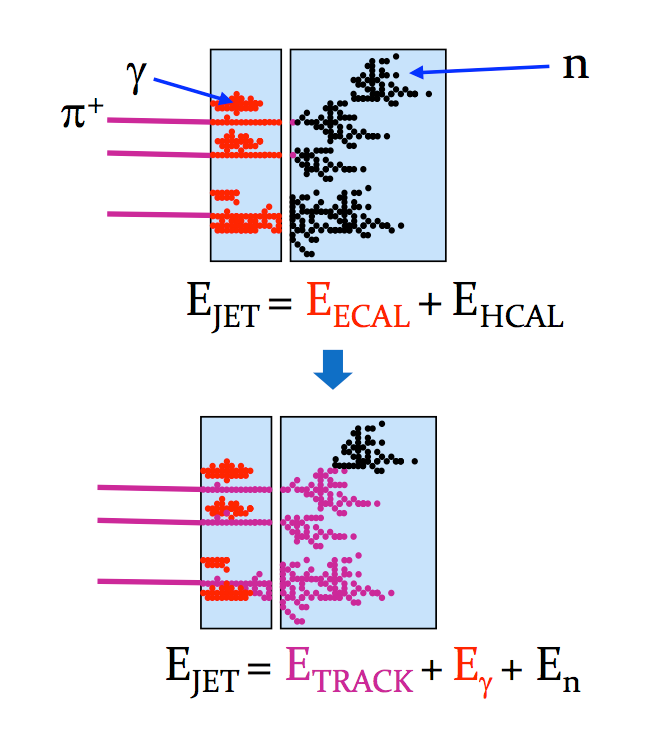
\includegraphics[scale=0.3]{PFlow.png} 
      \caption{Particle Flow Concept.}
   \label{fig:pflow}
\end{wrapfigure}

Concerning simulation, Particle Flow has been implemented known as Pandora PFA in full ILD simulation. One further approach is the use of fast simulation. Why using fast simulation? In simple words, it is much faster (for example, a ttbar event takes few seconds compared to minutes in full simulation). Like that several studies could be done much faster than when using full simulation, and variation of observables much easier while keeping a precision close to the full simulation. \\

Currently, several fast detector simulation exist of different types or methods. SGV (Simulation a Grande Vitesse) is one of them which is developed by Mikael Berggren, it is a fast detector simulation program using covariance matrix calculations. The status of SGV is that it performs already very well compared to full simulation and also integrates a Particle Flow Parametrisation in order to simulate Pandora PFA \cite{Berggren}.\\

My studies will focus on the performance of SGV compared to full simulation and also the Particle Flow parametrisation performance in SGV. The motivation is to show that SGV perform as well as the full simulation (benchmark of SGV) and to improve the current Particle Flow parametrisation. 

\section{Pandora Particle Flow Algorithm}

Pandora PFA is a very complex algorithm developed by M.A Thomson at the University of Cambridge. The following paragraphs will describe key steps that Pandora do in order to reconstruct ParticleFlow Objects (PFOs) or commonly Reconstructed Particles. 

\subsection{Key steps in the algorithm}

The algorithm is composed a several key steps to reconstruct particles \cite{Pandora}:

\begin{figure}[H]
\centering
   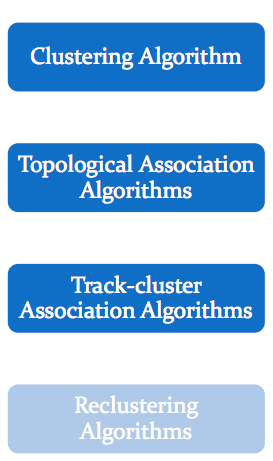
\includegraphics[scale=0.3]{steps.png} 
      \caption{Pandora PFA key steps.}
   \label{fig:pflow_step}
\end{figure}

\noindent
\begin{itemize}
\item Clustering: Cluster Calorimeter hits together taking into account several hit parameters (position, direction, density, energy...) and topological associations of clusters.
\item Track-Cluster Matching: Tracks and Clusters are associated with topological parameters (direction of track, proximity of cluster...) and physical parameters (energy, type of cluster, distance between clusters, energy profile...).
\item Reclustering: Identify inconsistent Track-Cluster Matching and re-cluster these until matching seems most appropriate.
\item Photon recovery: Recover photons in clusters.
\item Fragment removal: Evaluate changes between track-cluster compatibility if nearby neutral cluster would be merged to a charged cluster.
\item PFO Construction: Forms Particle Flow Objects from final clusters using track and calorimeter information.
\end{itemize}

\subsection{Cluster formation}

Calorimeter cells are clustered using a cone-based algorithm from the front of the ECAL to the back of the HCAL. The seed can come from the projection of the inner detector track on the ECAL front face. 

\begin{figure}[!h]
   \centering
   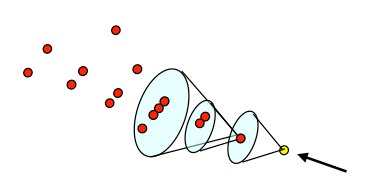
\includegraphics[scale=0.5]{clustering_cone.png} 
      \caption{Clustering.}
   \label{fig:clustering}
\end{figure}

A list of clusters is created by the algorithm then by iteration the algorithm adds hits to clusters and create a final list of clusters that can be modified later on by other algorithms. The cluster algorithm tends to split up the energy deposits from individual particles (rather than risking of accidentally merging in early reconstruction).
A topological algorithm takes the list of clusters and performs a check for particular topologies that can merge or modify existing clusters, no new clusters can be formed. 

\begin{figure}[!h]
   \centering
   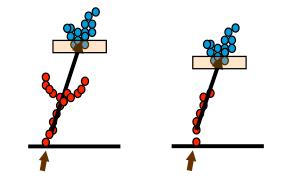
\includegraphics[scale=0.5]{topo_cluster.png} 
      \caption{Topological associations.}
   \label{fig:topo}
\end{figure}

\subsection{Track Matching}

After the clustering, calorimeter clusters are associated to tracks by comparing cluster properties like energy, direction with track properties (helix parameters, track state at the ECAL front face). This algorithm creates a proto-list of cluster-track associations. 

\begin{figure}[!h]
   \centering
   \includegraphics[scale=0.5]{track_cluster_asso.png} 
      \caption{Track Cluster association.}
   \label{fig:track_cluster_asso}
\end{figure}

\subsection{Statistical Reclustering}

The previous steps are found to perform very well for jet energy below 50 GeV. At higher energies, the resolution degrades due to an increasing overlap between hadronic showers. Such reconstruction failure can be found by comparing the cluster energy and the track momentum. 
If the energy of the calorimeter cluster does not agree with the momentum of the associated track, the cluster can be reconfigured in order to match to the track. 

\begin{figure}[!h]
   \centering
   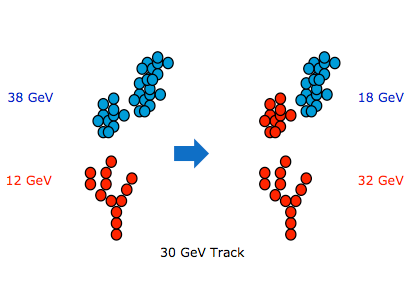
\includegraphics[scale=0.5]{reclustering.png} 
      \caption{Reclustering in case of bad matching.}
   \label{fig:reclustering}
\end{figure}

The cluster can pass through a series of configured clustering algorithm to see if a better track-cluster combinaison can be found. The cluster is going through the main clustering algorithm iteratively with a cone getting smaller until the cluster energy and the track momentum are compatible. If no improvement can be done, the original cluster is kept.

\section{Particle Flow in SGV}

Fast detector simulation exists of different types and different methods. For any of them, the goal is to be able to simulate the detector response with a time as the same order as to generate an event (order of 10 ms).
For this, a four smearing vector can be done assuming global detector properties. More elaborate, a parametric simulation (like SIMDET) can be done, where the response depends on the energy of the particle and its angle.
And finally, covariance matrix calculations can be done using the detector layout and the generated particles. SGV is found in this category \cite{Berggren}.

\subsection{Tracking in SGV}

A track is calculated by the intersection of the helix of a particle with pseudo-layers in the tracker. From the outermost hit, an helix is parametrised and then propagated to the next inner layer and the intersection and covariance matrix are calculated, the propagation is done until the inner most layer is reached. 

In SGV, there is no definition of hits. The helix is followed through the detector to find what pseudo-layers (tracker material is described by pseudo-layers) are hit by the particle. The tracking is done until the intersection of the start of the innermost calorimeter is reached. At each intersected pseudo-layers, the covariance matrix of the track is calculated.  The covariance matrix is translated along the trajectory and multiple scattering effects are included into calculation. 
In a basic view, it is what a Kalman filter is doing but not in the formal way. The track fitted is matched to the vertex and the perigee parameters are then smeared according to the calculated covariance matrix. The tracking efficiency has been parametrised from the full simulation.

\begin{figure}[!h]
   \centering
   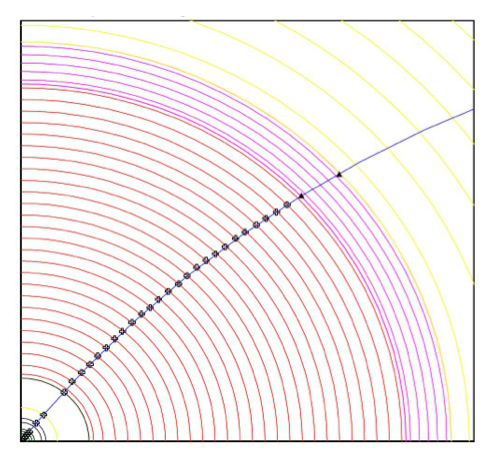
\includegraphics[scale=0.3]{Tracking_SGV.png} 
      \caption{Tracking in SGV. The tracker is represented by pseudo-layers at which intersection with a track, the covariance matrix is calculated, going from the outer part of the tracker to the inner part (inverse Kalman fitter).}
   \label{fig:tracking_sgv}
\end{figure}

\subsection{Calorimeter Simulation}

For the calorimeter simulation, the particle is extrapolated to the intersections with the calorimeters. At this point, a decision is made, that it should be detected as a minimum ionising particle, or that it should initiate an electromagnetic shower, or a hadronic shower, or that it is below the threshold... According to the decision, the detector response is simulated from different parameters (energy, type of particle, detector region...). Some parameters can be controlled by steering files, like shower can be merged if they are close to each others. To go towards more realism, the simulation of confusion between clusters can be done (Particle Flow simulation). 

\subsection{SGV Particle Flow parametrisation}
\label{sec:sgv_pflow}

Usual problems with fast simulation are already implemented in SGV: errors on detected energy, shower position and shape. However, there are association errors: Clusters might be merged, split or get associated to the wrong track. If (a part of) a neutral cluster is wrongly associated to a charged track (so then considered as a charged cluster), energy is then lost (Figure \ref{fig:asso_errors}). On the other hand, if (a part of) a charged cluster is not associated to any track (considered then as a neutral cluster), the energy is double counted (Figure \ref{fig:asso_errors2}). Theses mis-associations give rise to an error on the total energy of an event and the momentum \cite{Madalina}.

\noindent
\begin{minipage}{\linewidth}
\centering
\begin{minipage}{0.4\linewidth}
\begin{figure}[H]
   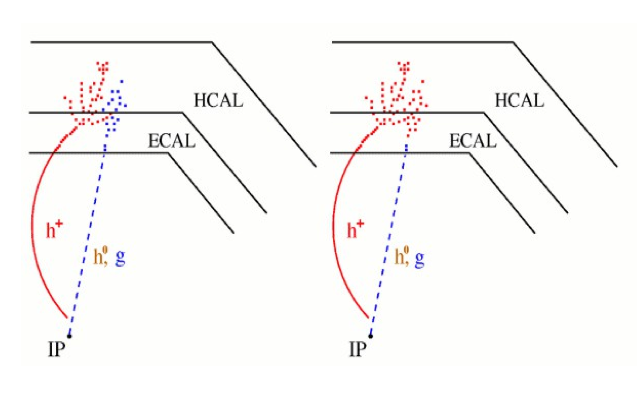
\includegraphics[width=\linewidth]{cluster_merge.png} 
    \caption{If the cluster is merged, energy is lost}
    \label{fig:asso_errors}
\end{figure}
\end{minipage}
      \hspace{0.05\linewidth}
      \begin{minipage}{0.4\linewidth}
\begin{figure}[H]
    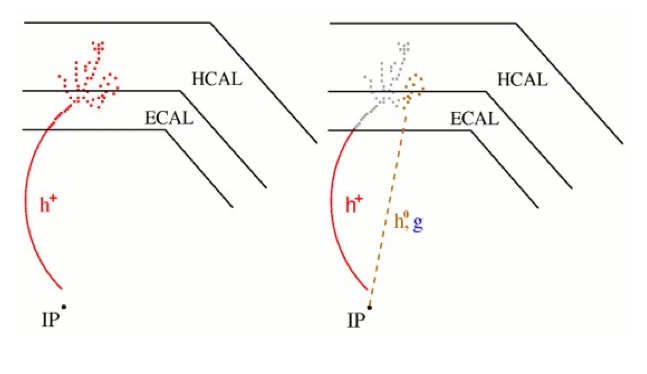
\includegraphics[width=\linewidth]{cluster_split.png} 
      \caption{If the cluster is split, energy is double-counted.}
   \label{fig:asso_errors2}
\end{figure}
\end{minipage}
\end{minipage}\\[0.4cm]

\noindent
The study of these association errors was done by using LOI mass produced samples from full simulation using the particle flow algorithm PandoraPFA  \cite{Thomson}. The most relevant observables were identified as: the cluster energy, the distance of the nearest particle of "the other type'' (i.e. neutral-to-charged or charged-to-neutral), whether the particle was a hadron or not, and whether it would be detected in the barrel or end-cap calorimeters.
The confusion was factorized in 4 sub-processes \cite{Berggren}:

\begin{itemize}
\item The probability of a cluster to split or merge (Figure \ref{fig:proba_split}).
\item In case of splitting, a probability to split off/merge the \textbf{entire} cluster.
\item In case of splitting but not completely, a function of the fraction of split off.
\end{itemize}
\begin{figure}[!h]
   \centering
   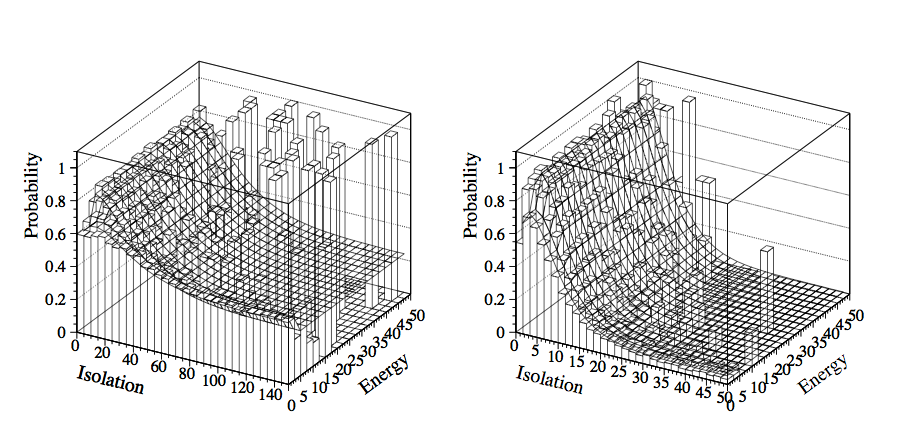
\includegraphics[scale=0.4]{prob_split.png} 
       \caption{Probability distribution of splitting in function of the cluster energy and the type of the particle.}
   \label{fig:proba_split}
\end{figure}

\noindent
\begin{minipage}{\linewidth}
\centering
\begin{minipage}{0.4\linewidth}
\begin{figure}[H]
   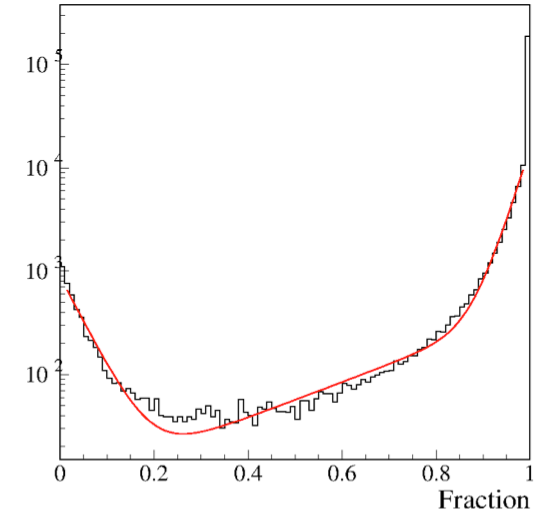
\includegraphics[width=\linewidth]{photon_loss_para.png} 
    \caption{Fitting of the probability of merging for photons.}
   \label{fig:proba_para}
\end{figure}
\end{minipage}
      \hspace{0.05\linewidth}
      \begin{minipage}{0.4\linewidth}
\begin{figure}[H]
    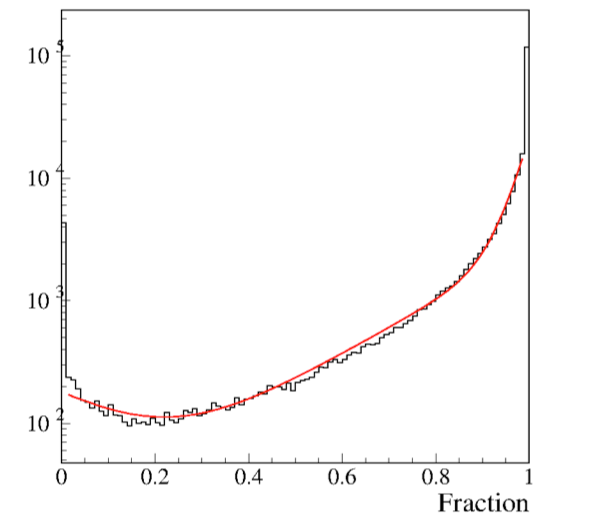
\includegraphics[width=\linewidth]{had_cha_dc_para.png} 
      \caption{Fitting of the probability of splitting for charged hadrons.}
   \label{fig:proba_para2}
\end{figure}
\end{minipage}
\end{minipage}\\[0.4cm]

\noindent
From this, probability distribution functions are derived (Figures \ref{fig:proba_para} and \ref{fig:proba_para2}). The algorithm is applied in the Particle Flow parametrisation of SGV. So far, the results seems to be in a good agreement mostly for the neutrals but still some development is needed to get the best agreement possible between SGV and the full simulation.

\subsection{Check Tracking efficiency SGV/Full simulation}
\label{sec:tracking}

Before reconstructing particles, PandoraPFA applies a selection of the tracks that can be a candidate to a reconstructed particle. In this tracking selection, 
PandoraPFA assumes that everything is a pion as a first guess. This is not modified after for track energy calculation. 

Particles coming from V0s (decay of a particle in flight for example $\gamma \rightarrow$ e$^+$e$^-$), Kinks (decay of a particle into another particle of the same charge with lower momentum giving a change in the curvature, for example $\pi \rightarrow \mu \nu$) or Prongs (decay of a $\tau$) are identified in a first place and treated separately.
Pandora PFA uses a track selection code in order to categorise them into multi parameters categories : 

\begin{itemize}
\item CanFormPFO
\item CanFormClusterlessPFO
\item CannotFormPFO
\end{itemize}

To perform the categorisation, PandoraPFA applies several cuts on the track. 
First, it checks the number of hits of the track in the tracking chamber (TPC) and the forward tracker (the number of hits in the TPC must be between 5 and 5000 hits, in the forward tracker, a number of expected hits is calculated based on the geometry of the forward tracker if tan $\lambda$ of the track is within the acceptance of the forward tracker). 

Then, Pandora checks if the track reaches the front face of the electromagnetic calorimeter. The conditions are that the radius of the outermost hit or the max z position of all hits is above a minimum radius (R$^{SET}_{min}$) or minimum z (Z$^{ETD}_{min}$), or if there is a sufficient number of hits in the TPC (11) or FTD (4). If the track has a low transverse momentum (meaning that the track may curl inside the inner tracker), that the cosine angle of the track is within the acceptance of the TPC or that the transverse momentum of the track is above a threshold (0.3*B*R$^{TPC}_{outer}$/2000).

If the track survive all these cuts, a quality check is performed on the tracks parameters: curvature ($\Omega$), impact parameter (d$_0$), z position at the p.c.a (z$_0$), radius of innermost hit ($r_{min}$) and the track energy (E$_{track}$). The curvature must be different from 0, the momentum uncertainty $\sigma_p$/p must be under 15\%. If the track momentum p is over 1 GeV, the transverse momentum p$_T$ and the momentum projected on the z axis p$_Z$ must be different of 0 GeV and finally the number of TPC or FTD hits must be over a certain value (for TPC hits, an expected number of hits is calculated based on the geometry and the track momentum and compared to the number of measured TPC hits, for FTD hits, the number must be more than 2 hits).

Once a track passes the quality checks, Pandora categorise the track on cut based differentiation. If a track has  d$_0 <$ 50 mm, z$_0 <$ 50 mm and $r_{min}$  $<$ $R^{TPC}_{inner}$ + 50 mm, the track is then categorised as \textbf{CanFormPFO}. 

A second criterion is used for non vertex tracks (tracks that are not matching the primary vertex), a check on $z_{min} - z_0$ ($z_{min}$ is the z position of the first tracker hit) and the $r_{min}$ of the track is done. If the track passes through the cuts, it is flagged also as \textbf{CanFormPFO}. 

\begin{figure}[!h]
   \centering
    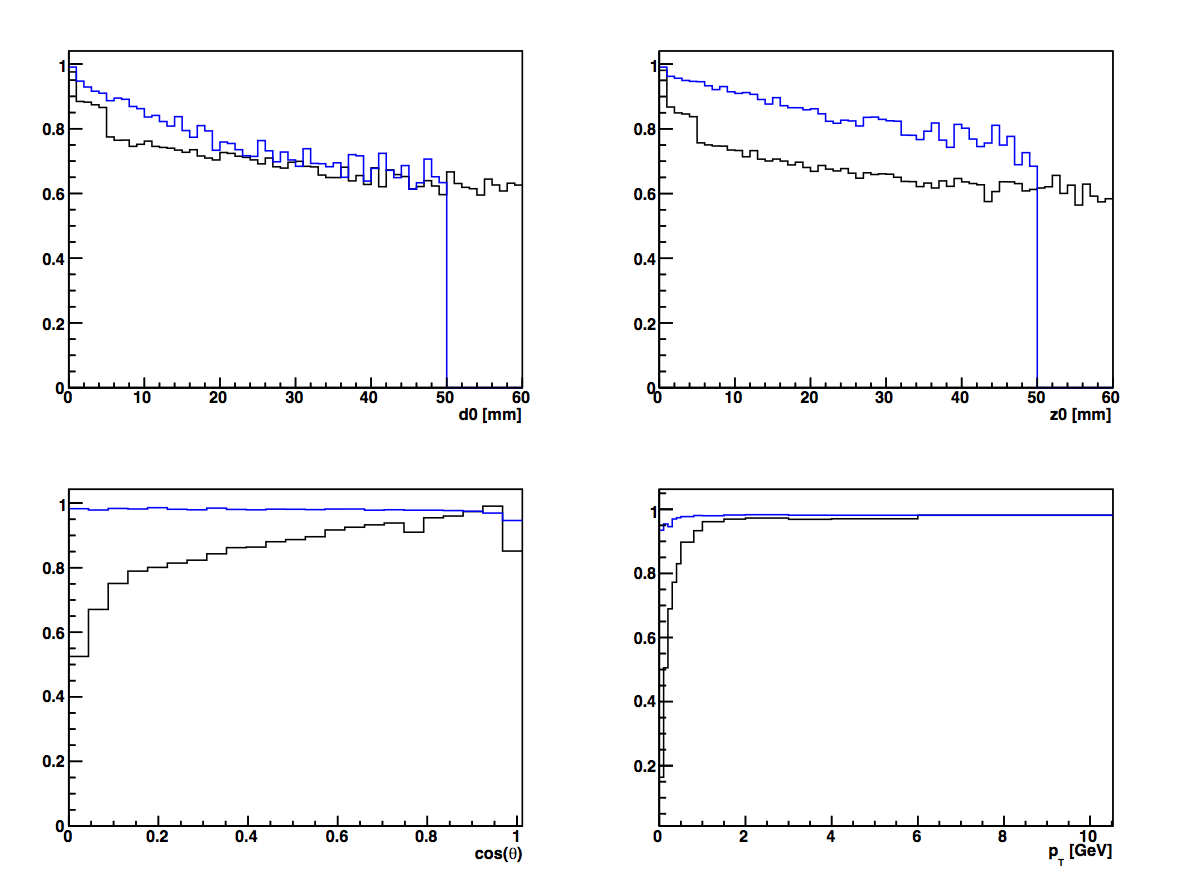
\includegraphics[scale=0.5]{eff_track_selection_curlers.png} 
      \caption{Ratio plots for different track parameters for full simulation in black and SGV in blue.}
   \label{fig:trk_select_wcurlers}
\end{figure}

If a track (unmatched vertex track) has d$_0 <$ 5 mm, z$_0 <$ 5 mm, $r_{min}$  $<$ $R^{TPC}_{inner}$ + 50 mm and the track energy E$_{track}$ is less than 5 GeV, the track is then categorised as \textbf{CanFormClusterlessPFO}. For obvious reasons, tracks matching these criteria can end up in the category \textbf{CanFormPFO}. This is then disentangled later by the track - cluster matching. 
For tracks that are in the first steps categorised as V0s, Kinks or Prongs are also flagged as \textbf{CanFormPFO} or \textbf{CanFormClusterlessPFO} depending on the same criteria above.

All the others tracks that do not meet the criteria are then flagged \textbf{CannotFormPFO}, theses tracks will then not form any PFO in the reconstruction.

The goal was to check if whether Pandora rejects tracks with a PFO in SGV. As in SGV, no information is provided on the state of the track at a specific point or no tracker hit information is stored, only the relevant part of the selection made by PandoraPFA was applied. After the pseudo-selection, histograms (h$_{selected}$) for each track parameter (d$_0$, z$_0$, cos($\theta$) and p$_T$) were filled. For tracks that have the flag 'inPFO" (meaning that the track was indeed used by Pandora and formed a PFO), histograms (h$_{inPFO}$) with the track parameters were also filled.

To compared the performance of SGV to full simulation, a ratio was defined as the ratio of h$_{inPFO}$ / h$_{selected}$ for the full simulation. In SGV, all tracks are by default forming a PFO, with the selection a certain number of tracks might not pass thus with the ratio definition above, it might be over 1. In that case, for SGV, the ratio was defined as h$_{selected}$ / h$_{inPFO}$.
We obtain the plots shown in Figure \ref{fig:trk_select_wcurlers}:

As expected for the full simulation, the impact parameter (d$_0$) and the z position at the p.c.a (z$_0$) ratio plots are more or less constant, as for SGV it seems to drop but the influence in general is not a problem. For the $p_{T}$ plot, SGV seems to have a better ratio, but this is more or less dependant on the geometry parametrisation of SGV which is relevant for low $p_{T}$ particles. The main difference appears for the $cos(\theta)$ parameter, the full simulation seems to drop very much for very low angles compared to SGV. After further investigation, theses tracks are curlers in the TPC that make through until the endcap, at this reconstruction step, theses tracks are considered by Pandora to be able to form a PFO but further a matching between clusters and track enables to get rid of most of theses curlers. By introducing a harder cut for theses curlers, basically looking at the $z_{min}$ - z$_0$ ($z_{min}$ is the z position of first hit) that should be less than half a turn of the helix. We obtain the plots shown Figure \ref{fig:trk_select_wocurlers}:

\noindent
\begin{minipage}{\linewidth}
\centering
\begin{minipage}{0.4\linewidth}
\begin{figure}[H]
    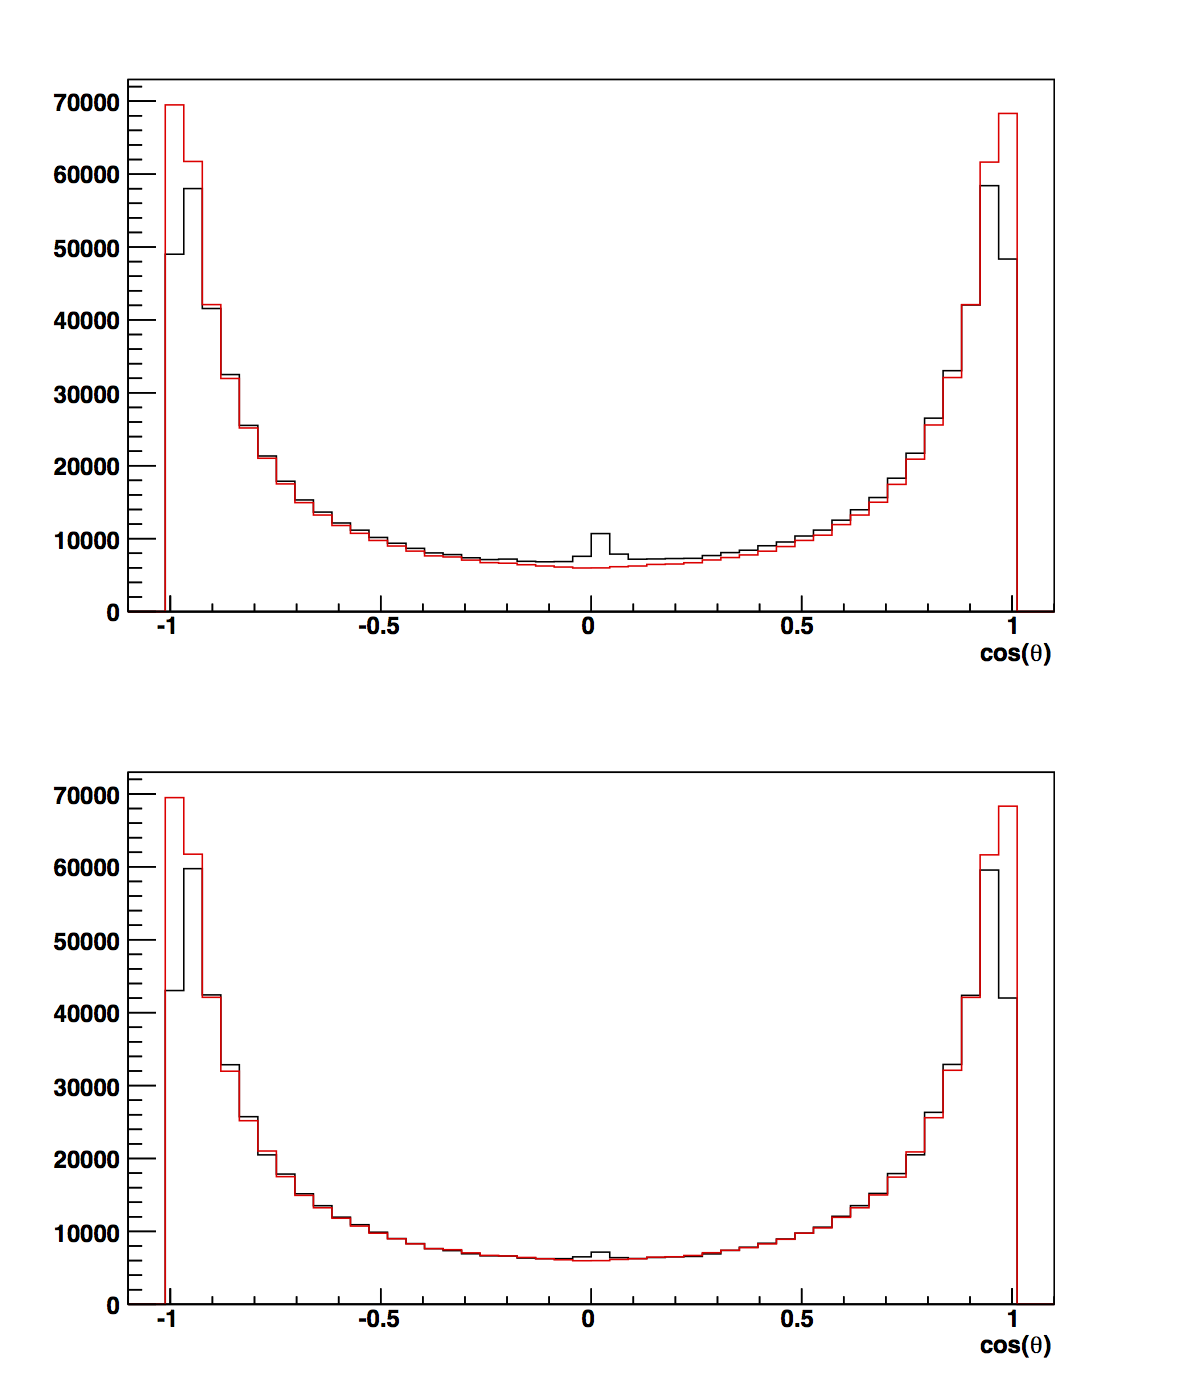
\includegraphics[width=\linewidth]{Comp_alltrk_Pandoratrk_toMC_wocurlers.png} 
 \caption{$cos(\theta)$ distribution for MC tracks and Pandora tracks after the selection and with harder cut on $z_{min}$.}
   \label{fig:trk_para_mc_reco}
\end{figure}
\end{minipage}
      \hspace{0.05\linewidth}
      \begin{minipage}{0.4\linewidth}
\begin{figure}[H]
    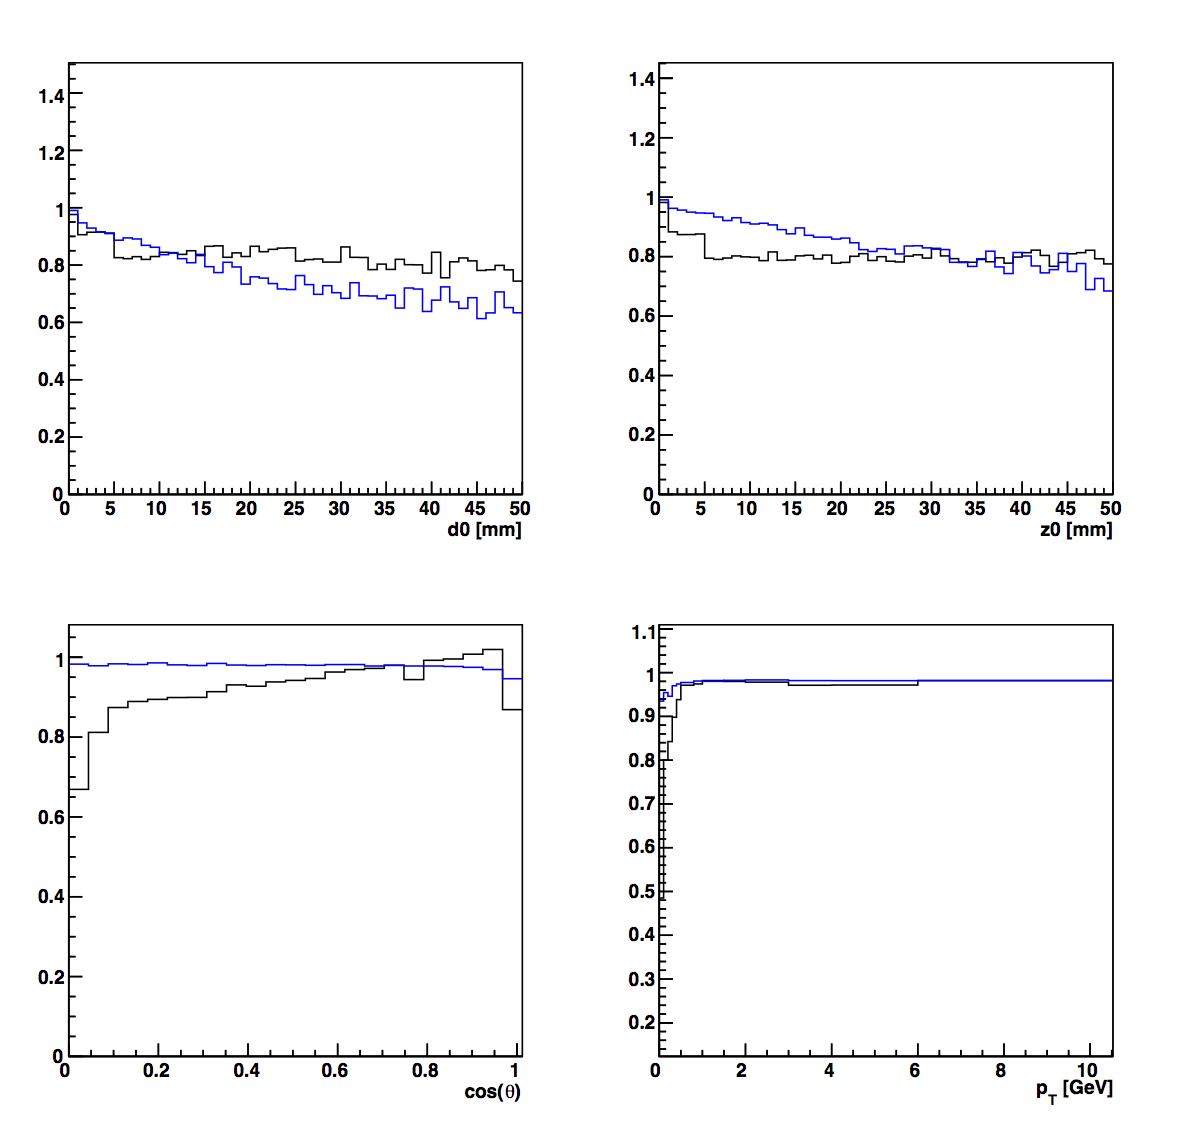
\includegraphics[width=\linewidth]{eff_track_selection_wocurlers.png} 
 \caption{Ratio plots of the track parameters after getting rid of most of the curlers.}
   \label{fig:trk_select_wocurlers}
\end{figure}
\end{minipage}
\end{minipage}\\[0.4cm]

\noindent
One can see that after SGV and full simulation agrees more after this harder cut. The cut seems still not enough to get rid of most of the curlers looking at the $cos(\theta)$ distribution. From this, one can say that the tracking selection in PandoraPFA is not responsible for the observed discrepancy. 

\subsection{Track Multiplicity and Correlations}

A look at the number of tracks or multiplicity inside a jet was performed in order to see if SGV performs as expected in full simulation. The number of tracks were counted per jet energy bins for full simulation, SGV with and without ParticleFlow as shown on Figure \ref{fig:trk_multiplicity}. 

\begin{figure}[!h]
   \centering
    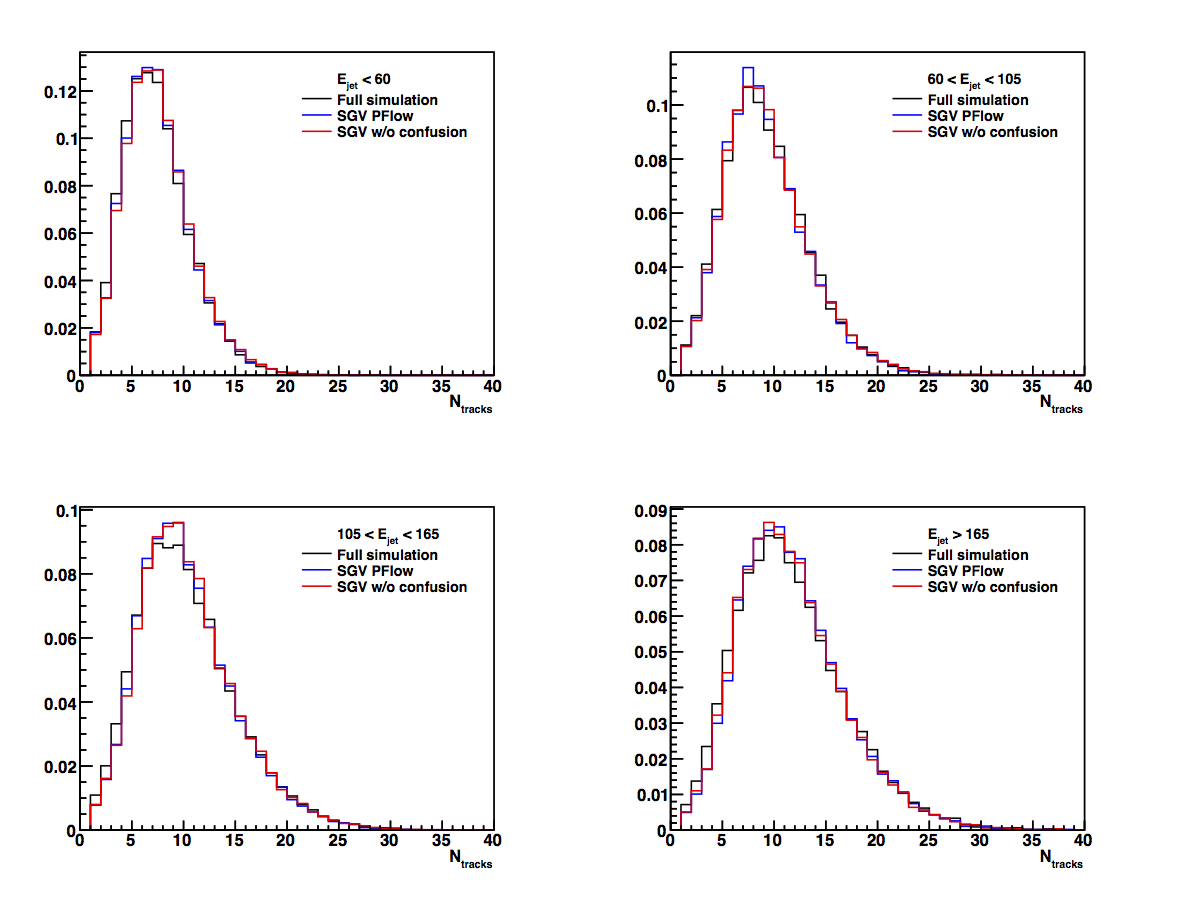
\includegraphics[scale=0.5]{multiplicity_jet_track.png} 
      \caption{Track Multiplicity for SGV and full simulation. The results are in a very good agreement.}
   \label{fig:trk_multiplicity}
\end{figure}

One can see that the multiplicity of tracks are in very good agreement between SGV and full simulation. This is not the only variable that we looked at. Typically inside a jet, 60-70\% is composed of charged particles and 20-30\% of neutrals (neutrons and photons), thus the correlation between charged/neutral energy and track multiplicity was also looked at. The distributions shown on Figure \ref{fig:correlation_distrib} are in agreement and correspond to what one can expect.

\noindent
\begin{minipage}{\linewidth}
\centering
\begin{minipage}{0.4\linewidth}
\begin{figure}[H]
    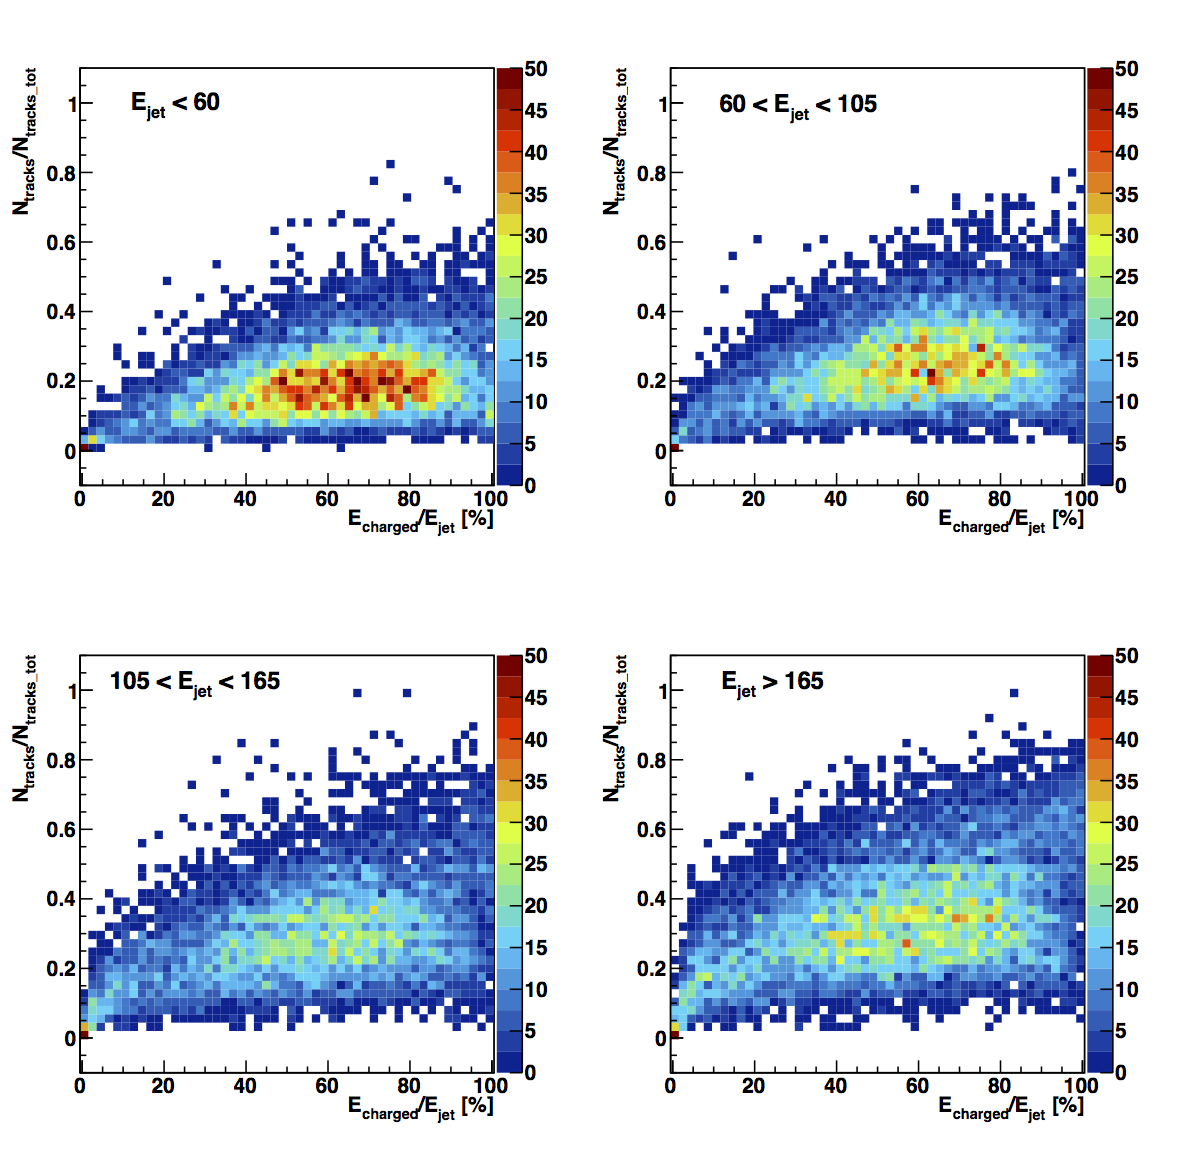
\includegraphics[width=\linewidth]{Correlation_Ntrack_FracEchajet_full.png}
\end{figure}
\end{minipage}
      \hspace{0.05\linewidth}
      \begin{minipage}{0.4\linewidth}
\begin{figure}[H]
    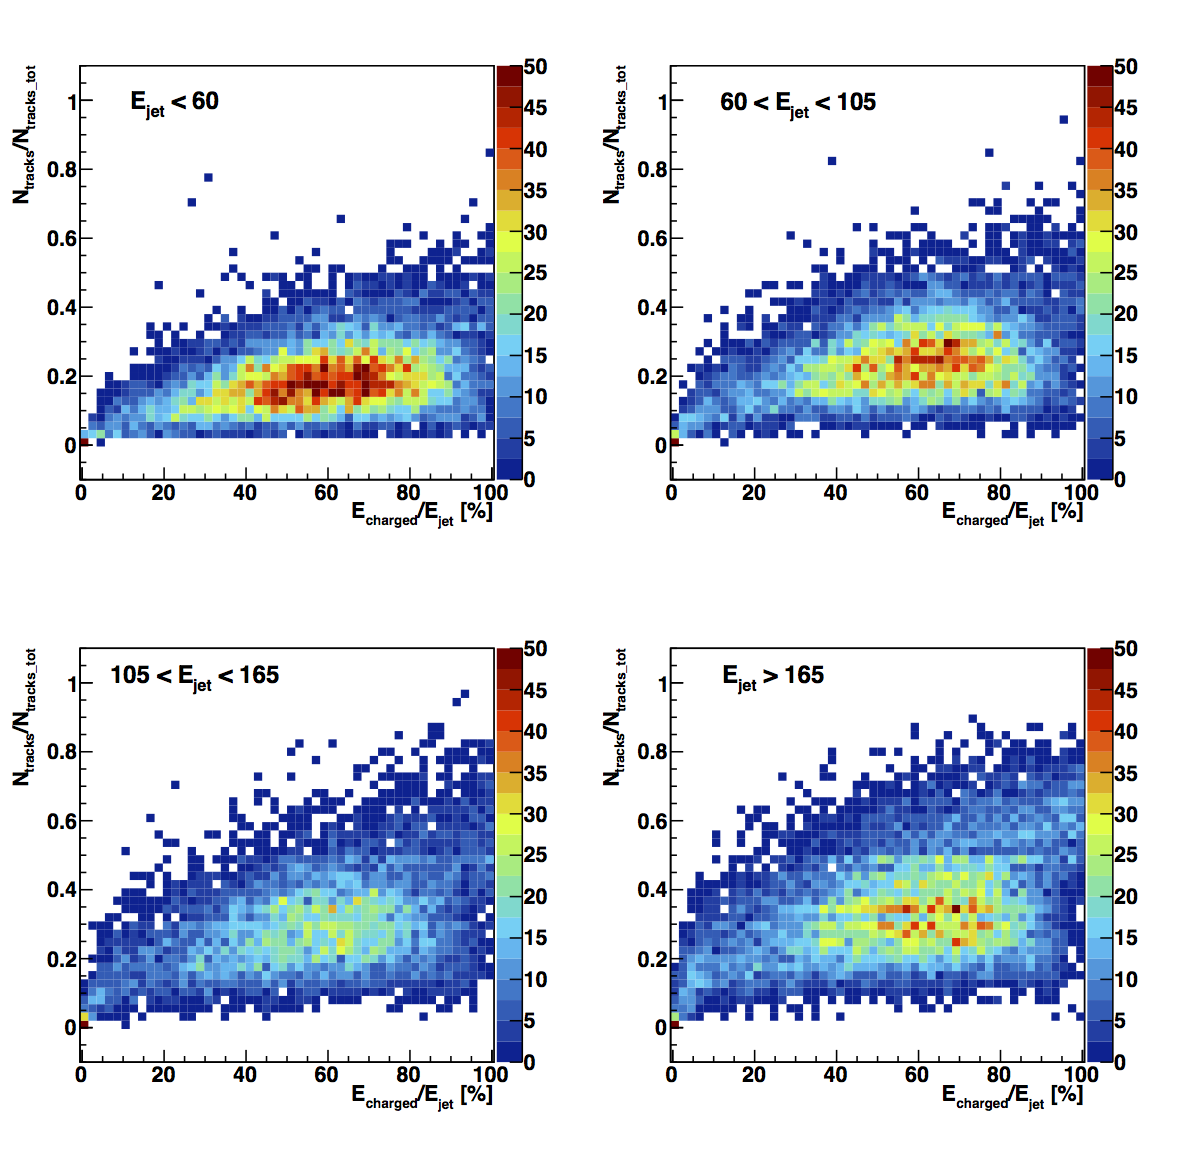
\includegraphics[width=\linewidth]{Correlation_Ntrack_FracEchajet_sgv.png}
\end{figure}
\end{minipage}
\captionof{figure}{Correlation track multiplicity normalised to the total number of tracks versus the charged energy normalised to the jet energy for different jet energy bins. On the left in full simulation, on the right in SGV.}
   \label{fig:correlation_distrib}
\end{minipage}\\[0.5cm]

\section{Particle Flow studies}

\subsection{Double counted and lost energy}

Association errors can happen during reconstruction as explained in section \ref{sec:sgv_pflow} because of a confusion term (the confusion is that sometimes it is very difficult to say from which particle a cluster is coming from, then a cluster is a sum of particle contributing with different weight to the cluster energy) coming from the overlap of showers into the calorimeters. 

\begin{figure}[!h]
   \centering
   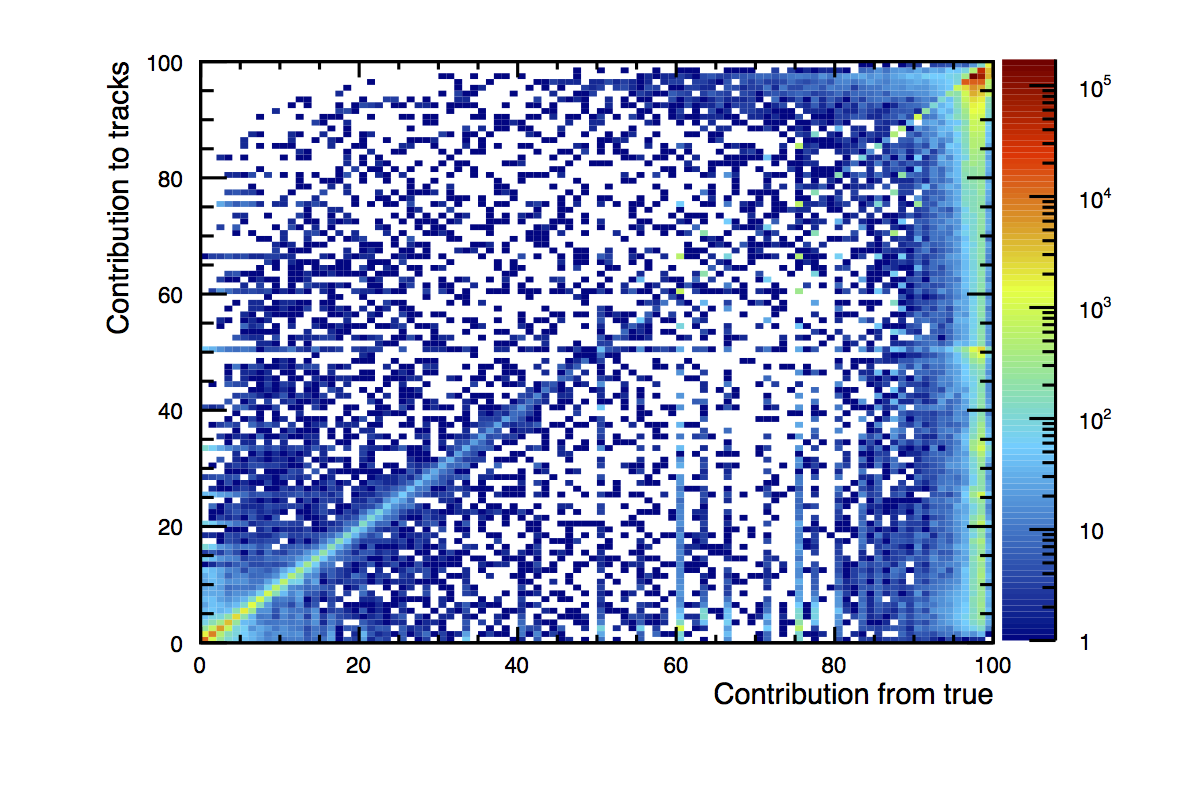
\includegraphics[scale=0.5]{weight_corr.png} 
      \caption{Distribution of the weights of track-true particle relation. The contribution from true represent the contribution of a true particle (in terms of hits from this true particle compared to the total hits in the track) to a track, and the contribution to track represent the inverse relation, e.g. the number of hits from a true particle compared to the total of simulated hits from this true particle.}
   \label{fig:weight}
\end{figure}

On Figure \ref{fig:weight}, there are mainly 2 regions, the top right corner and the bottom left corner. The top right corner represents the region where there is almost no confusion between a track and the Monte-carlo particle (or true particle) associated (there is almost a one-to-one relation between a track and a true particle, e.g, one true particle is associated to a track). The bottom left corner is the region where the confusion dominates, this region shows that it is difficult to associate correctly a particle to a track, the contributions seems to come from different particles.

The goal of particle flow is to avoid confusion as much as possible. There can be different points of view concerning the treatment of the double counted and lost energy: 
\begin{itemize}
\item At a cluster-track level, by comparing the energy of a track (momentum + assumption of $\pi$ mass) to the energy of the cluster associated to the track (it would be then an energy flow point of view).
\item At a jet level (clusters contained into a jet of particles), by looking at the double counted and lost energy over the jet energy.
\end{itemize}

For characterising the particle flow parametrisation performance of SGV compared to the full simulation, a DBD sample was taken. The process chosen: $e^+e^- \rightarrow W^+W^- \rightarrow q\bar{q} q\bar{q}$ at $\sqrt{s}$ = 500 GeV, is particularly interesting in order to evaluate the separation between the two W bosons and the full hadronic decay complicating the reconstruction. 

\subsubsection{At Cluster-Track level}

At a cluster-to-track point of view, the following method has been pursued. For each event, each reconstructed particle is taken, then we look at the track associated to it and calculate the track energy as $E_{track} = \sqrt{\|\overrightarrow{p}\| \cdot \|\overrightarrow{p}\| + m_{\pi} \cdot m_{\pi}}$ with $m_{\pi}$ = 0.139 GeV and $\overrightarrow{p}$, the reconstructed particle momentum (the pion assumption is made like in PandoraPFA which in most cases is not wrong) [\ref{sec:tracking}]. Then we looked at the cluster associated to the reconstructed particle, and took the energy of the cluster $E_{cluster}$. A comparison between the track energy $E_{track}$ and the cluster energy $E_{cluster}$ is done. 

If $E_{track} < E_{cluster}$, the difference is counted as double counted energy (naturally the energy of the cluster should be the track energy because the resolution of the tracker is much better than the calorimeter, so if there is more energy in the cluster it means that a part of it might come from a near neutral particle or from a mis-measurement). If the opposite, then it is counted as lost energy. The double counted and lost energy is summed up for all the particles in the event.This method is done for each reconstructed particles in an event, thus for each event we have a point $E_{dc}$ and $E_{l}$. The result is shown in Figure \ref{fig:cluster_track_level}.

\begin{figure}[!h]
   \centering
   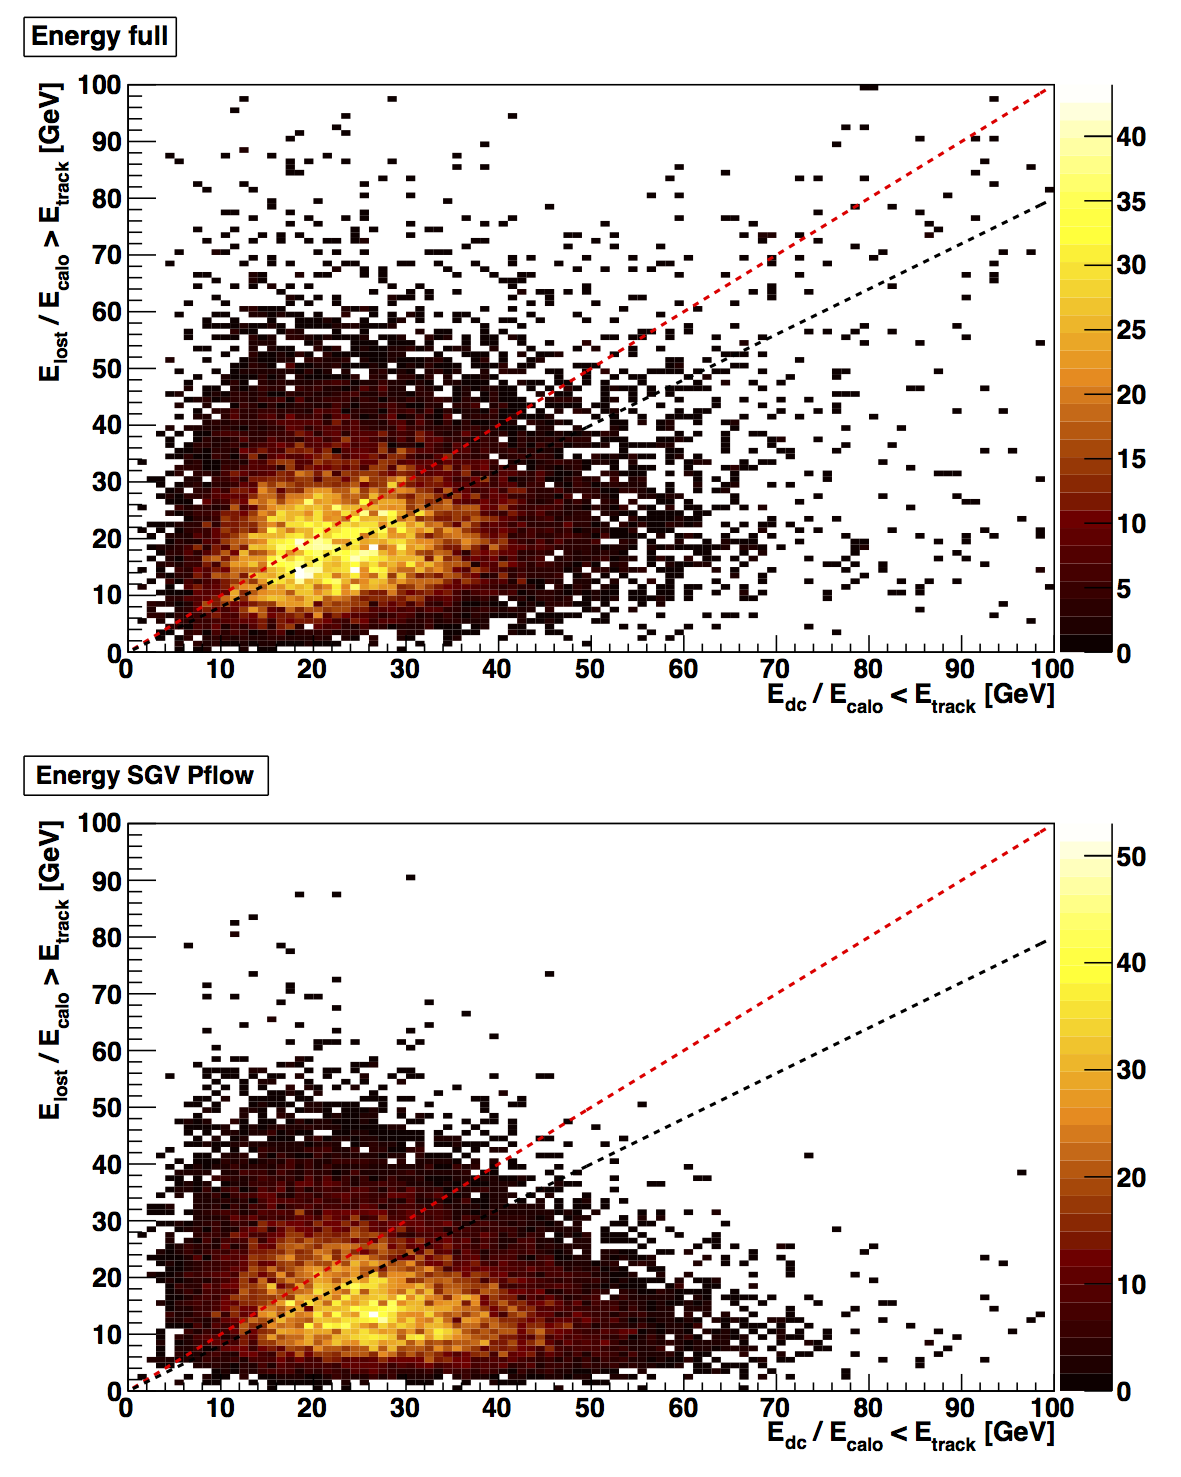
\includegraphics[scale=0.4]{Correlation_nojet.png} 
      \caption{2D plot representing the lost energy versus the double counted energy in a full simulation of $e^+e^- \rightarrow q\bar{q} q\bar{q}$ sample at $\sqrt{s}$ = 500 GeV. Each point in this plot represent an event. The red and the black dotted line represent a correlation of 100\% and 80\%. One can observe that there is different correlations for SGV and the full simulation.}
   \label{fig:cluster_track_level}
\end{figure}

Concerning the full simulation, it seems that Pandora is compensating between the lost and double counted energy. One can think that Pandora balances both quantities event by event. For SGV, the correlation is not bad with the parametrisation but seems still to differ from the full simulation, one can see that SGV is more double counting energy than losing energy. 

\begin{figure}[!h]
\centering
    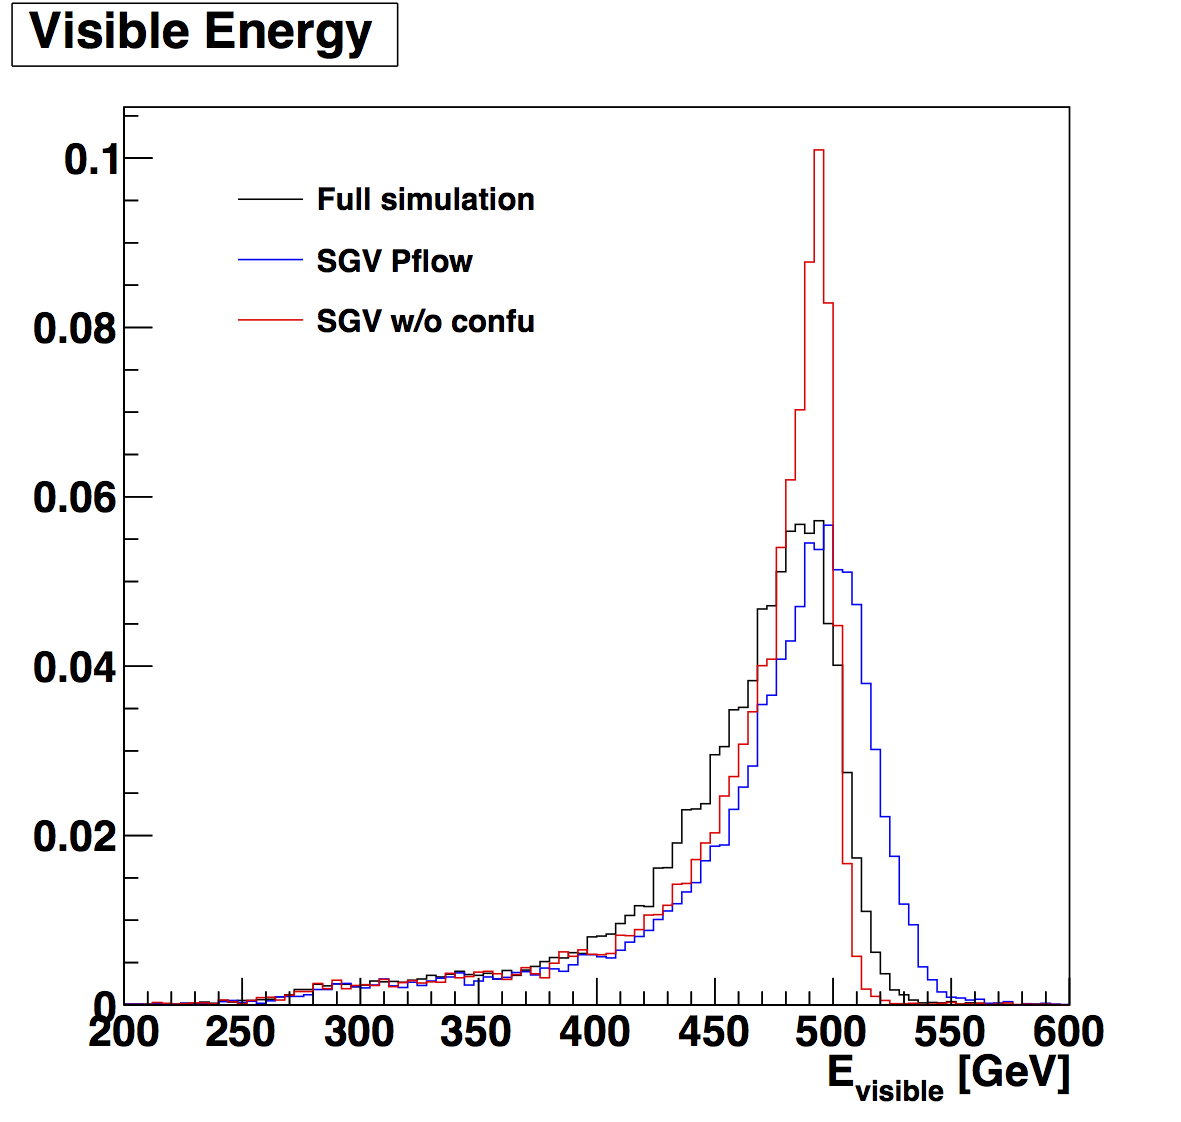
\includegraphics[scale=0.4]{Evis.png} 
    \caption{The plot represent the total energy or all the events for the full simulation and SGV with and without the particle flow parametrisation.}
   \label{fig:energy}
\end{figure}

On the total energy (Figure \ref{fig:energy}), SGV without confusion seems to describe well the total energy but doesn't include the reconstruction effects widening the distribution. When the confusion is turned on, a tail in the total energy appears and is not in accordance to the full simulation but the width of the distribution seems to be the same, it is then just a shift in energy. Thus, we looked at the energy distribution of neutral and charged reconstructed particles (Figure \ref{fig:energies2}). 

\begin{figure}[!h]
   \centering
  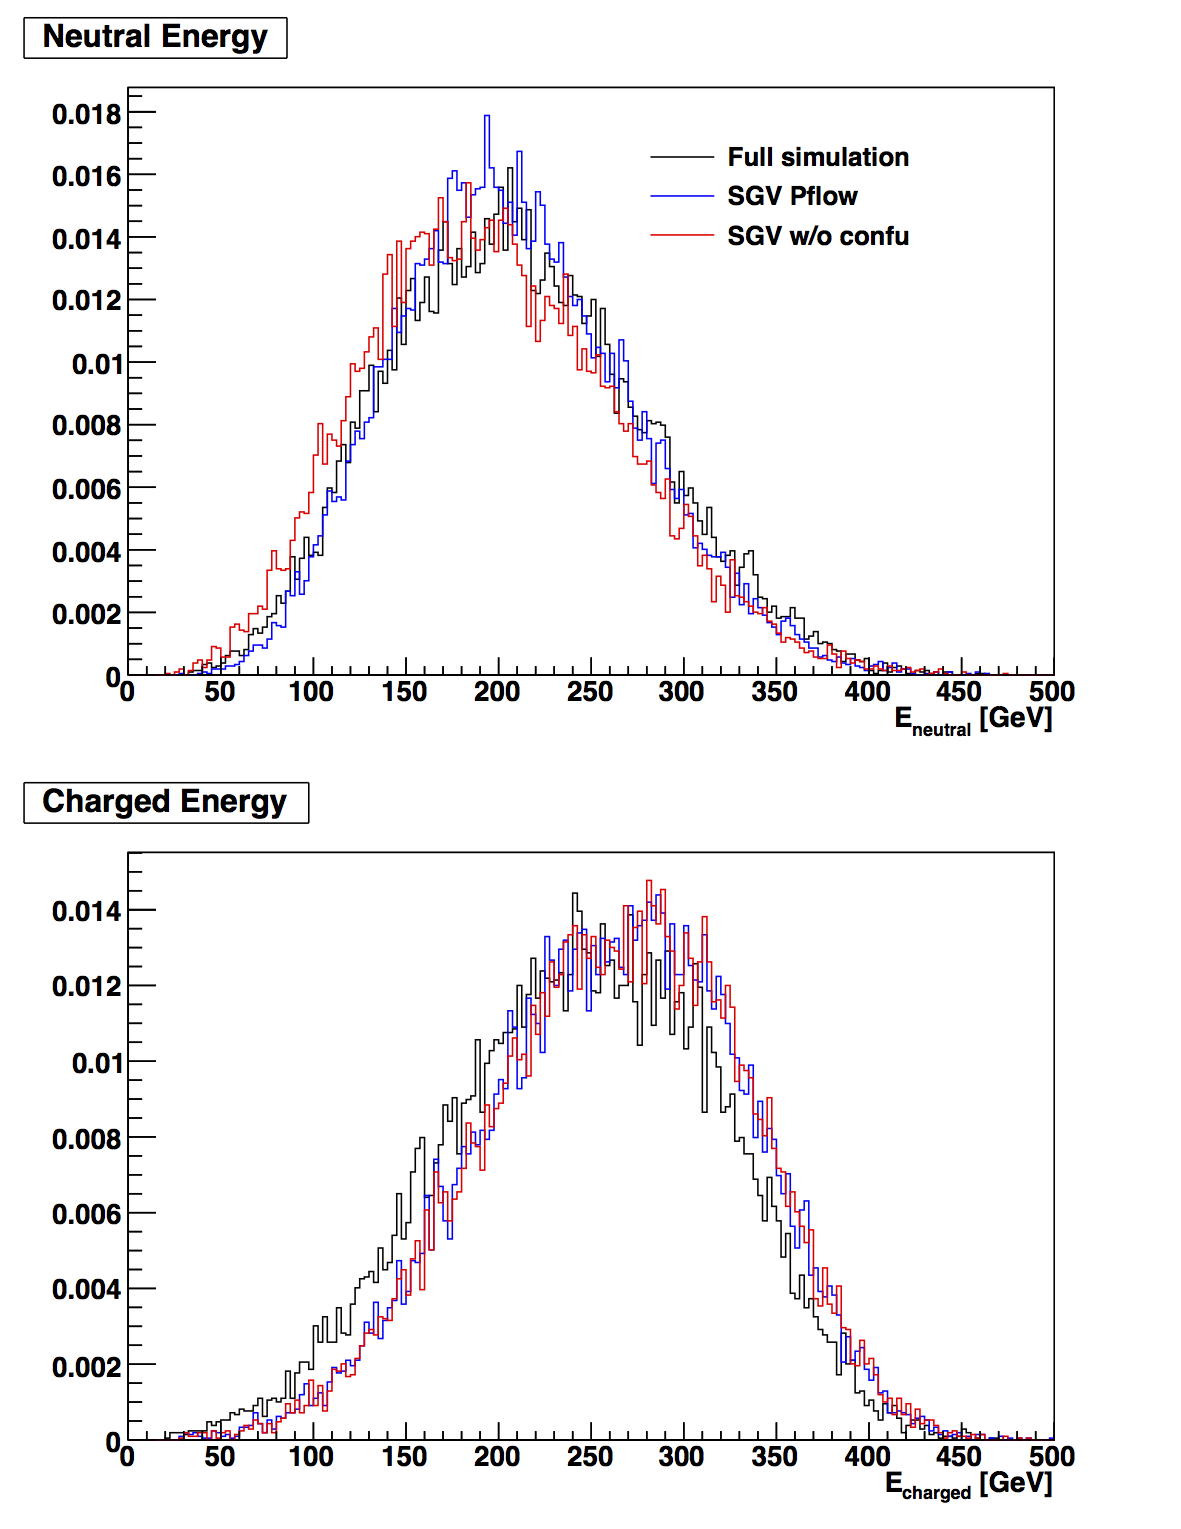
\includegraphics[scale=0.5]{Total_EneuEcha_notjet.png} 
      \caption{Charged and Neutral energies distributions for SGV (with and without Particle Flow) and full simulation.}
   \label{fig:energies2}
\end{figure}

The neutral distribution improves in SGV with the particle flow parametrisation and agrees well with the full simulation, but for the charged distribution, one can see that the confusion doesn't change anything (as expected because only the track information matters and the cluster is not related to it) and as expected the distribution is shifted to higher energies explaining the tail observed in the total energy distribution. This gives us a hint that the parametrisation should have an effect on the charged particles which can be possible in the case that the track information is rejected and only the calorimeter information is taken into account. 
Because of this, we decided to look at the same quantity but at the jet energy level, in order to see at what energy scale the discrepancy appears.

\subsubsection{At Jet level}

The process $e^+e^- \rightarrow q\bar{q} q\bar{q}$ at $\sqrt{s}$ = 500 GeV has a typical topology of 4 jets from the 4 primary quarks. The jets are obtained by running the Durham algorithm after the reconstruction. The Durham algorithm is a $k_T$-algorithm, it clusters all reconstructed particles into jets. 

First, jets are classified into few energy bins: 0 to 60 GeV, 60 to 105 GeV, 105 to 165 GeV and over 165 GeV. For each event, a jet is selected by different energy $E_{jet}$ :  $<$ 60 GeV, between 60 and 105 GeV, between 105 and 165 GeV and $>$ 165 GeV (Figure \ref{fig:jet_spec}). Inside each jet,  each reconstructed particle is taken. Then the same method as the section above is used. Now, we calculate E$_l$ and E$_{dc}$ per jet. At the end, the lost energy versus the double counted energy normalised to the jet energy (Figure \ref{fig:jet_track_level}).

\begin{figure}[!h]
   \centering
  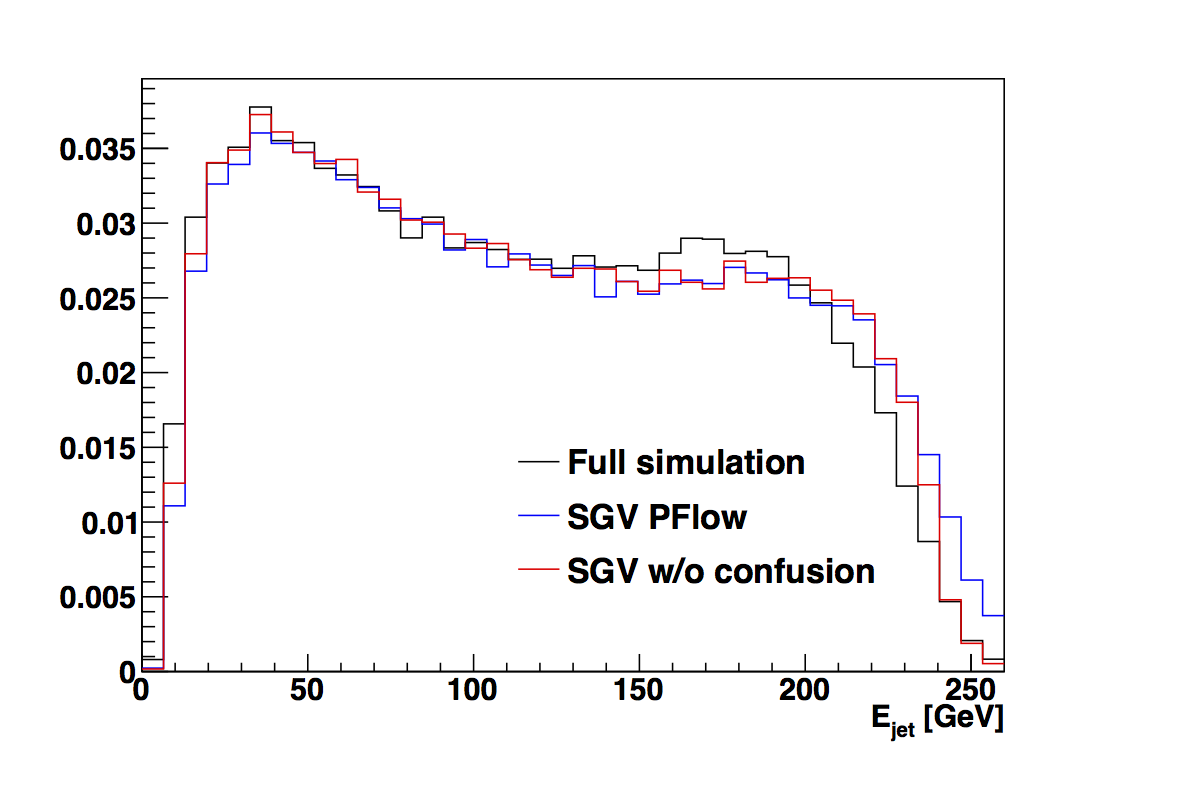
\includegraphics[scale=0.5]{Jet_spectrum.png} 
      \caption{Jet energy spectrum between full simulation and SGV. The jet energy bins were chosen in order to get the approximate same number of events in each bin.}
   \label{fig:jet_spec}
\end{figure}

One can see that for low jet energies, SGV and the full simulation seems to be quite in agreement. But the higher we go in jet energy, the more both are getting different. We can mostly see that for jet energies over 165 GeV, SGV is double counting much more than the full simulation which stays with a good correlation between $E_{dc}$ and $E_{l}$. This gives us indication that SGV is failing in regions where jet energies are high (around $>$ 165 GeV). 

The reason could be that, in theses cases, the energy density in the calorimeter is so high that the association errors can be committed more easily because the confusion term of the overlapping showers is getting bigger and bigger in function of the jet energy. PandoraPFA, to solve this problem, is switching to a pure "Energy Flow" mode. It is completely discarding the track information and only keeps the calorimeter information and then by reclustering, PandoraPFA is matching the overall energy in a calorimeter region to the tracks.

\noindent
\begin{minipage}{\linewidth}
\centering
\begin{minipage}{0.4\linewidth}
\begin{figure}[H]
    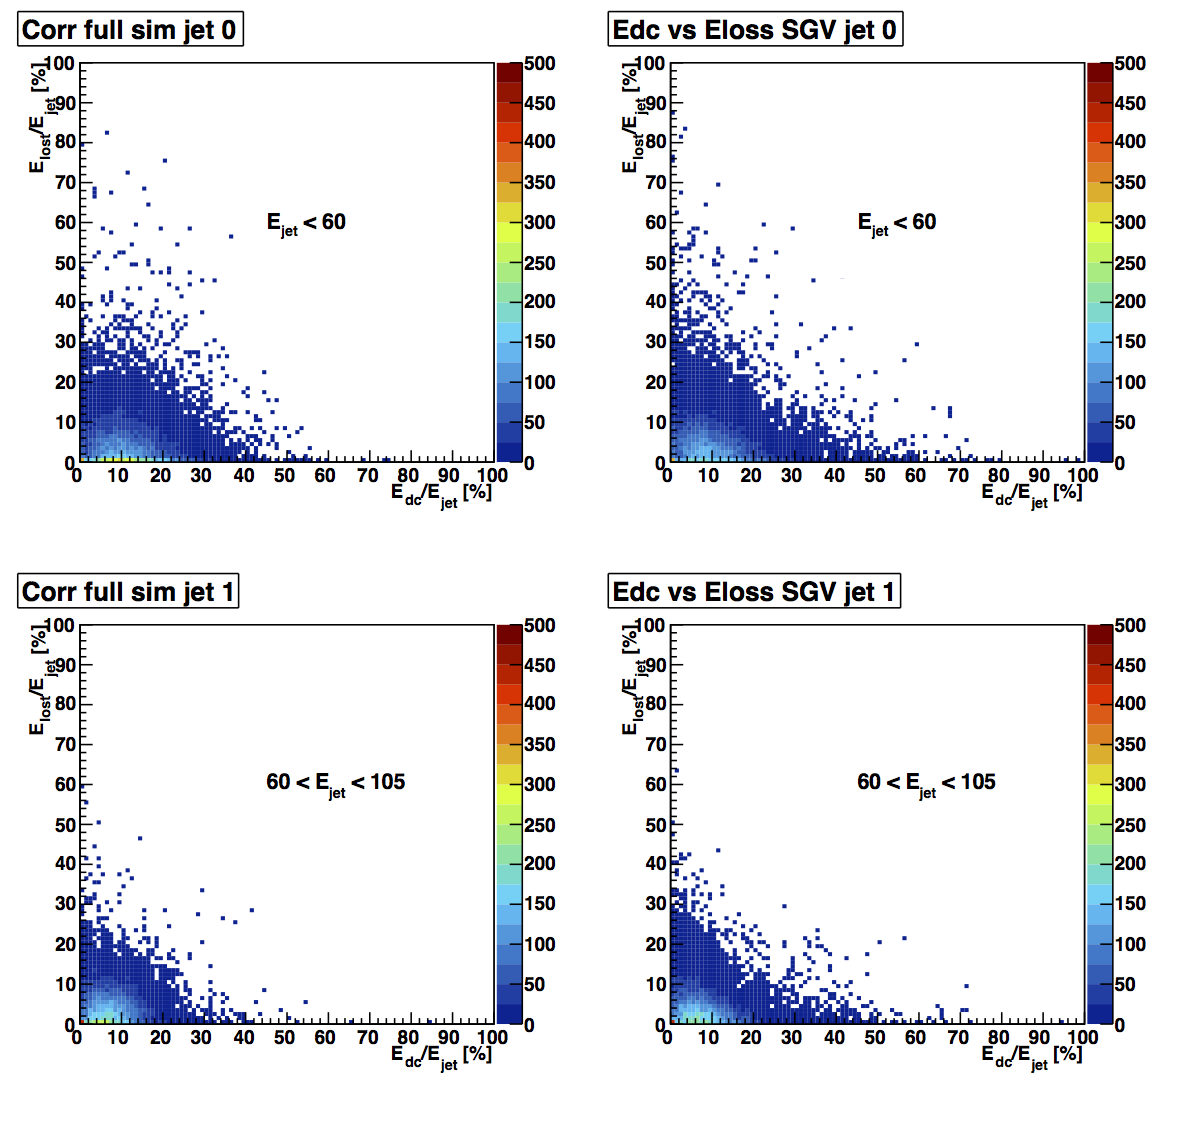
\includegraphics[width=\linewidth]{Correlation_1.png} 
\end{figure}
\end{minipage}
      \hspace{0.05\linewidth}
      \begin{minipage}{0.4\linewidth}
\begin{figure}[H]
    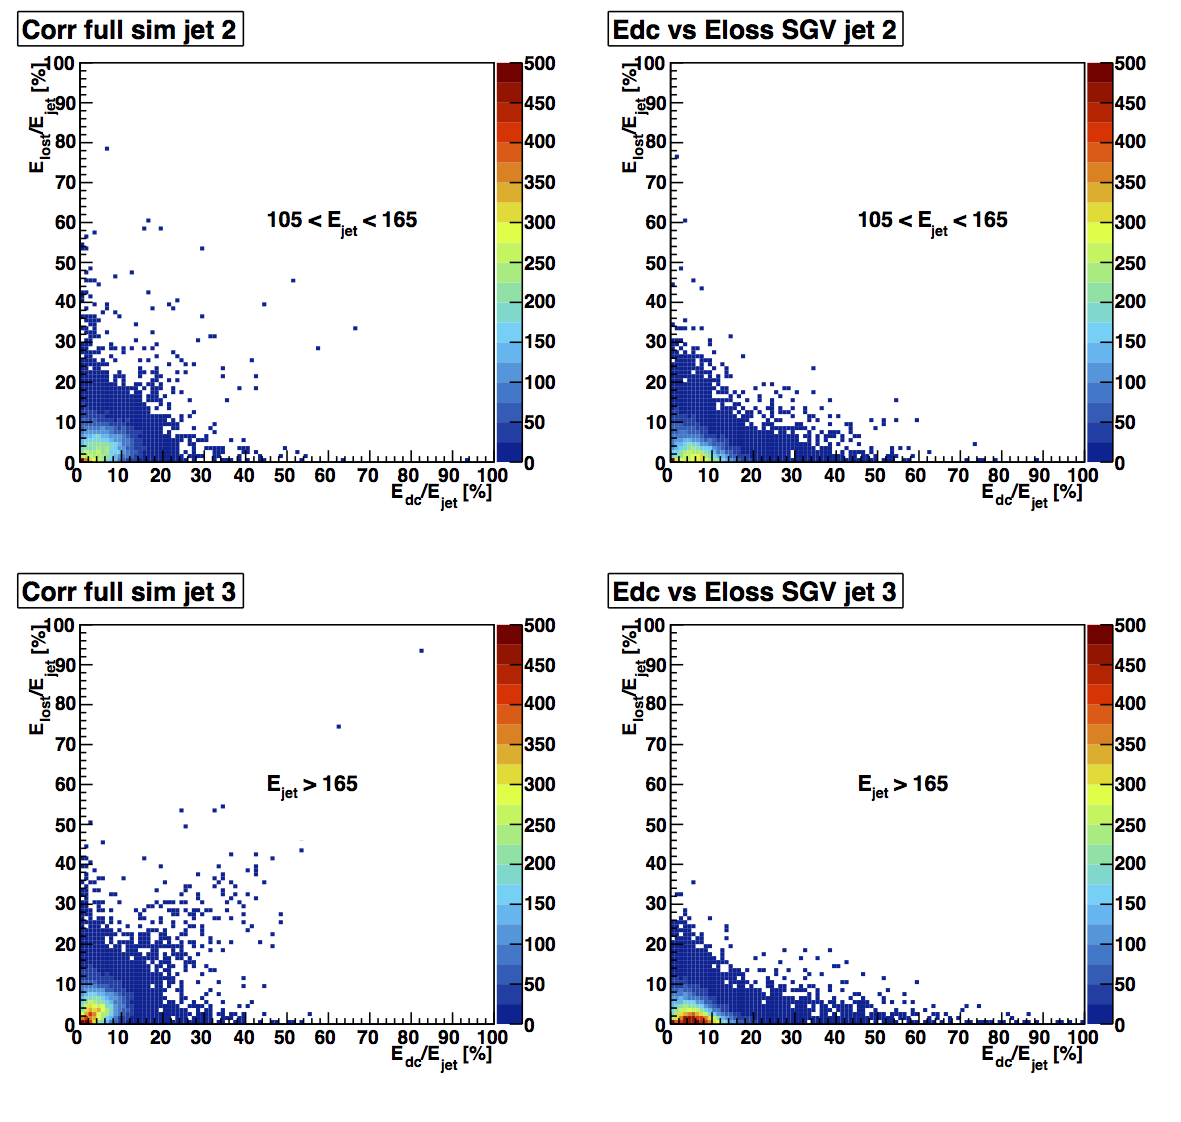
\includegraphics[width=\linewidth]{Correlation_2.png} 
\end{figure}
\end{minipage}
\captionof{figure}{Lost energy versus to the double counted energy normalised to the jet energy.}
   \label{fig:jet_track_level}
\end{minipage}\\[0.5cm]

In the current version of SGV, it is not implemented yet. We think that the merging and splitting probabilities should be then function of the energy density in the calorimeter region studied.

\subsection{Energy fraction}

The goal of this study was to look at the energy distribution for each jet energy bins. It can give us a clear view on the shape of the distribution and the effect of the particle flow parametrisation on it.

\noindent
\begin{minipage}{\linewidth}
\centering
\begin{minipage}{0.4\linewidth}
\begin{figure}[H]
    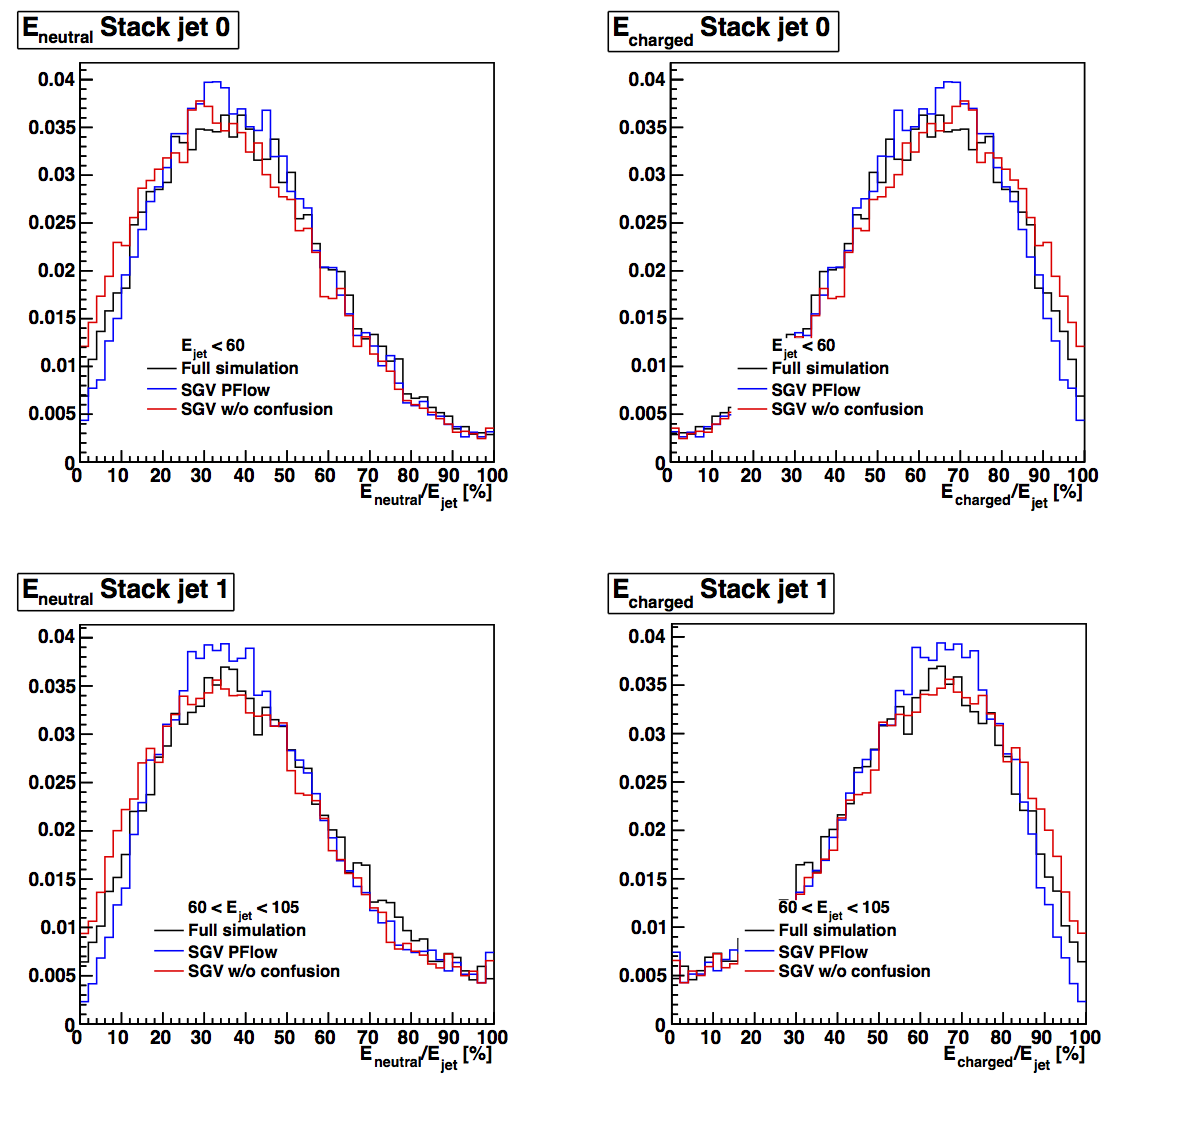
\includegraphics[width=\linewidth]{EneuEcha_binned_1.png}
\end{figure}
\end{minipage}
      \hspace{0.05\linewidth}
      \begin{minipage}{0.4\linewidth}
\begin{figure}[H]
    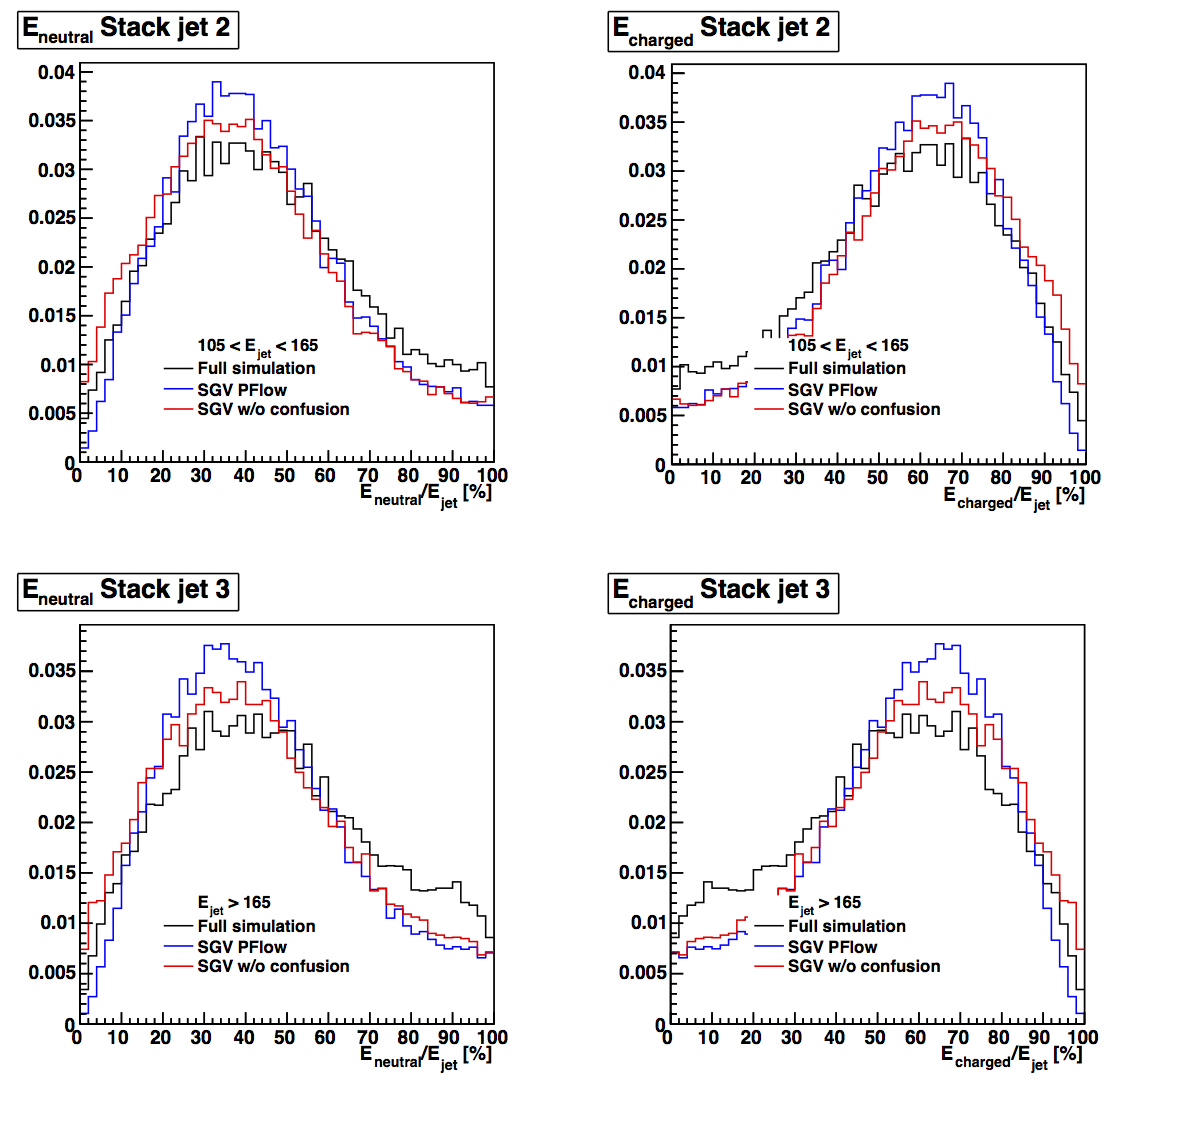
\includegraphics[width=\linewidth]{EneuEcha_binned_2.png} 
\end{figure}
\end{minipage}
\captionof{figure}{Energy distribution for charged and neutrals normalised to the jet energy.}
   \label{fig:energy_distrib}
\end{minipage}\\[0.5cm]

For the energy distribution plots on Figure \ref{fig:energy_distrib}, one can observe that the plots of neutral and charged energy are mirror to each other, as the sum of the charged and neutral energy should be equal to the jet energy. For low energy jets, the distributions seems to be rather in a good agreement, only small discrepancies are visible. For higher energy jets, this discrepancy is getting bigger. It seems that there is more energy in the 50-70\% region and much less in the 10-20\% region. It seems that SGV is pulling the energy in the wrong direction.

The idea is that charged energy from the 50+\% region should be transferred to the 10-20\% region, meaning that charged clusters are transformed to neutral clusters. That is how the total charged energy distribution could be shifted toward lower energies by "losing" charged energy and gaining neutral energy. This is consistent with the assumption that PandoraPFA is switching to an energy mode. It can occurs during this process that charged cluster are transformed to neutral cluster in order to match the E/p locally. PandoraPFA only takes care of the calorimeter information and reject the track information.

\subsection{Occupancy and Energy density}

One relative variable in the splitting and merging probabilities is the distance between a cluster of one type (hadronic or EM) and a cluster of the other type. The study of the distribution of the distance to the nearest neighbour was performed distinguishing between ECAL and HCAL (basically EM and hadronic showers). The procedure is perform such as: in each jet, a list of neutral and charged particles is filled. Each of theses particles are projected either on the barrel or the endcap respectively of the ECAL or the HCAL. The projection is done in order to calculate distances on the same geometry planes (SGV and the full simulation have a slight different geometry, the Barrel in SGV is considered as a cylinder of radius of the ECAL). 

After that, we take each neutral and calculate the 3D distance: $r_i = \sqrt{x_i^2 + y_i^2 + z_i^2}$ with $x_i$, $y_i$, $z_i$ the coordinates of the particle i intersected to the endcap or the barrel approximated to a cylinder of radius of the ECAL to each charged particles distinguishing between endcap and barrel to get rid of corner effects. The minimum distance $d_{min}$ defined as min($r_i$) for each neutral is then filled into an histogram, meaning there is an entry for each neutral particle. We obtain the plots shown on Figure \ref{fig:dmin}.

\noindent
\begin{minipage}{\linewidth}
\centering
\begin{minipage}{0.4\linewidth}
\begin{figure}[H]
    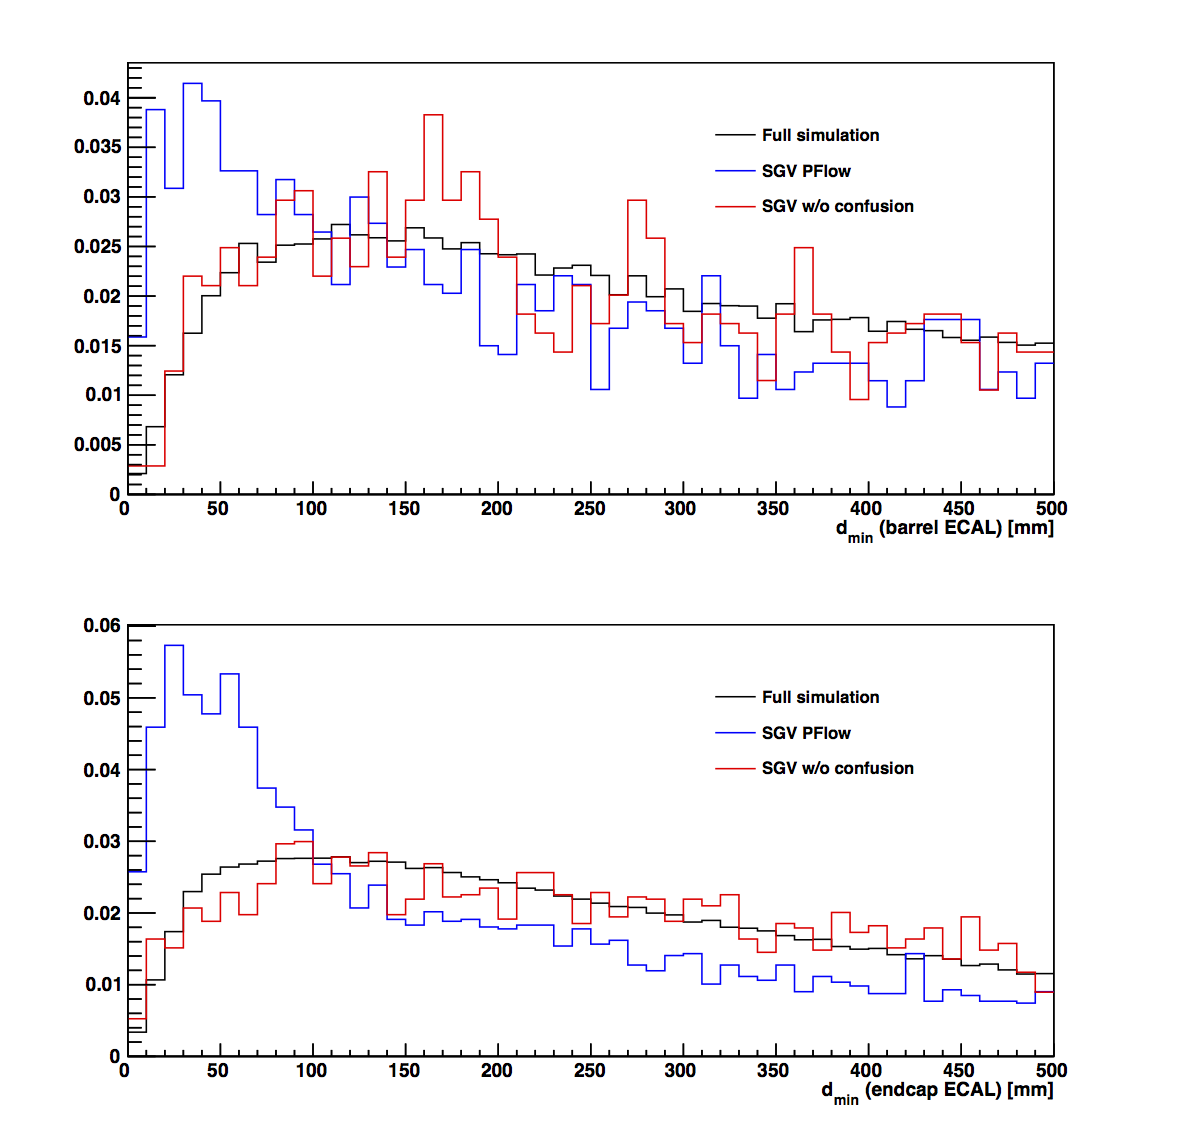
\includegraphics[width=\linewidth]{dmin_charged_to_neutral_ECAL_all.png}
\end{figure}
\end{minipage}
      \hspace{0.05\linewidth}
      \begin{minipage}{0.4\linewidth}
\begin{figure}[H]
    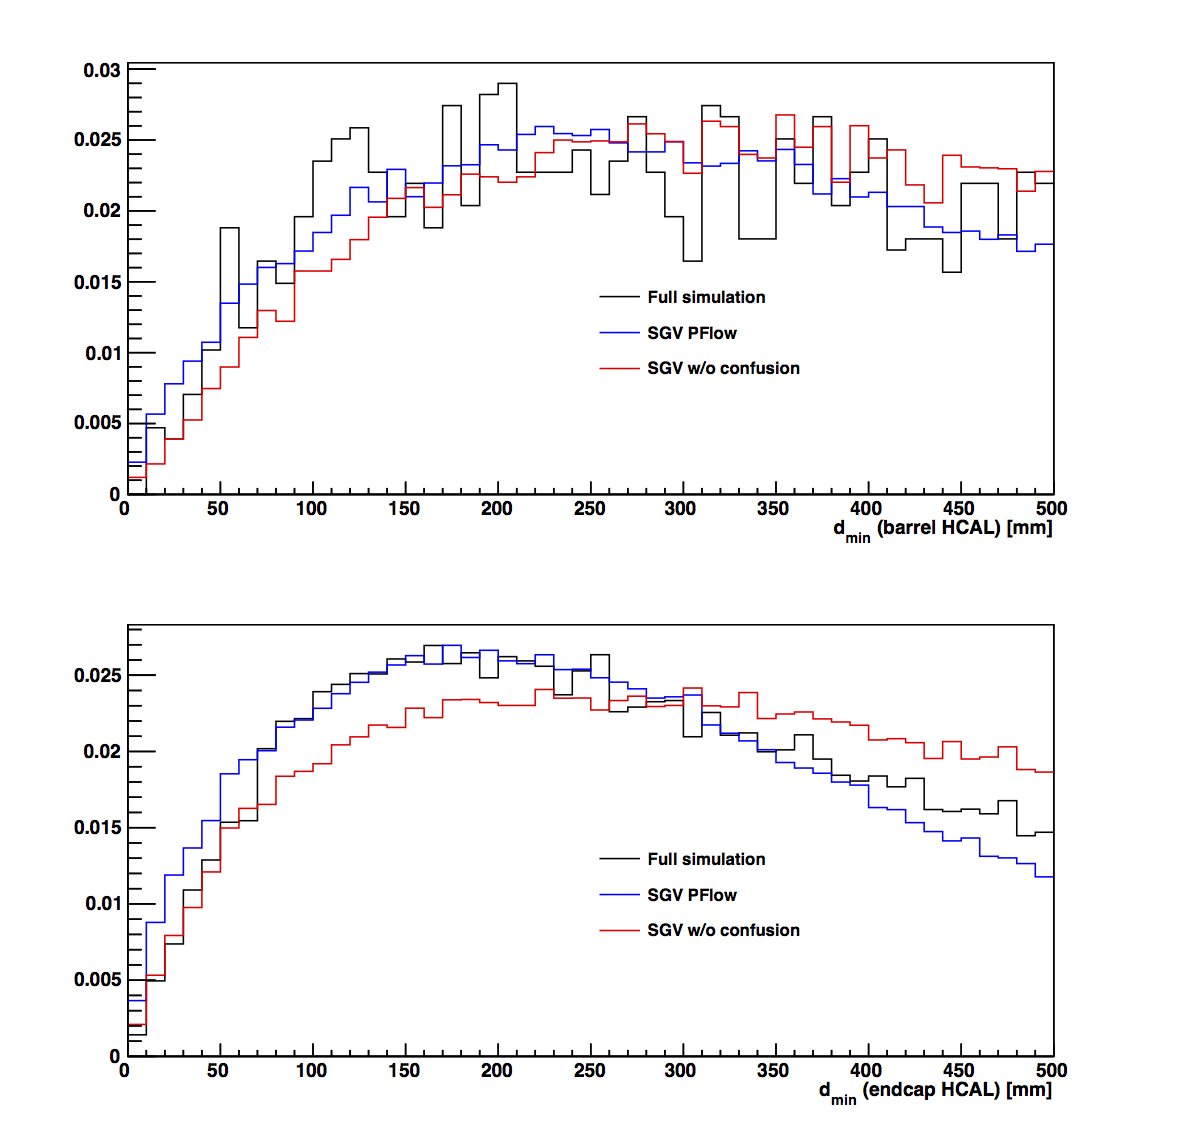
\includegraphics[width=\linewidth]{dmin_charged_to_neutral_HCAL_all.png} 
\end{figure}
\end{minipage}
\captionof{figure}{Distance to the closest charged distribution for the ECAL on the left and the HCAL on the right.}
   \label{fig:dmin}
\end{minipage}\\[0.5cm]

One can observe that there is a discrepancy between full simulation and SGV with Particle Flow in the ECAL. The Particle Flow parametrisation seems to have the effect that particles are placed closer in the ECAL. On the other hand, the Particle Flow parametrisation seems to have a rather good effect in the HCAL. The idea then was to "disable PFA" for the ECAL and look at the same distributions shown of Figure \ref{fig:dmin_2}.  

\noindent
\begin{minipage}{\linewidth}
\centering
\begin{minipage}{0.4\linewidth}
\begin{figure}[H]
    \includegraphics[draft,width=\linewidth]{dmin_ECAL_2.jpg}
\end{figure}
\end{minipage}
      \hspace{0.05\linewidth}
      \begin{minipage}{0.4\linewidth}
\begin{figure}[H]
    \includegraphics[draft,width=\linewidth]{dmin_HCAL_2.jpg} 
\end{figure}
\end{minipage}
\captionof{figure}{Distance to the closest charged distribution for the ECAL with Particle Flow parametrisation "disable" on the left and the HCAL on the right.}
 \label{fig:dmin_2}
\end{minipage}\\[0.5cm]

In that case, we could observe that the distributions are in rather good agreement for the ECAL and HCAL. The Particle Flow parametrisation seems to have a rather limited effect on the ECAL distribution compared to SGV without Particle Flow. 

Is the parametrisation of Particle Flow in SGV useless for the ECAL? In order to check the influence of the parametrisation on the ECAL energy distribution, the charged and neutral energy were looked at again. As expected, switching off the Particle Flow parametrisation for the ECAL have rather no or limited impact on the charged energy distribution as shown on Figure \ref{fig:energy_ECALnoPFA}.

\begin{figure}[!h]
   \centering
    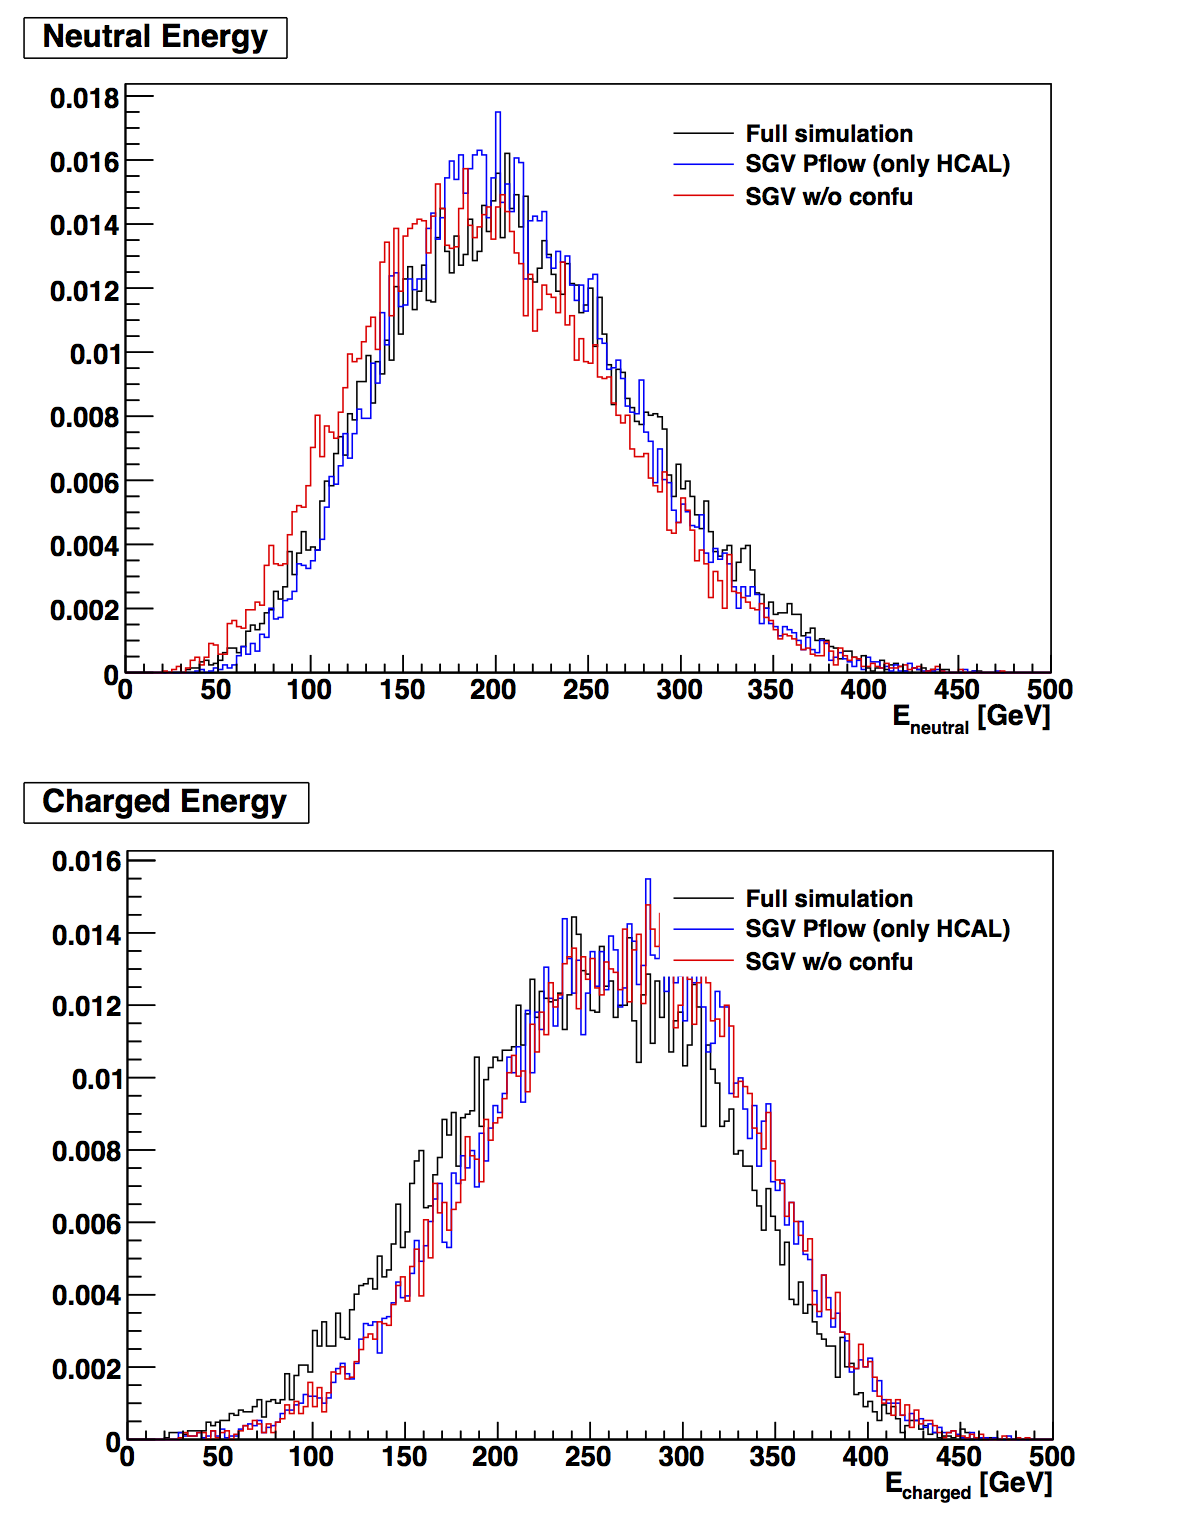
\includegraphics[scale=0.5]{Total_EneuEcha_notjet_onlyHCAL.png}
      \caption{Neutral and Charged energy distributions with ParticleFlow "disabled" for the ECAL.}
   \label{fig:energy_ECALnoPFA}
\end{figure}

One variable to look at would be the occupancy of the detector in the jet region or the energy density. This is could give us a clue to understand how PandoraPFA is splitting and merging in function of the energy density and then implement or correct the splitting and merging probabilities used in SGV to parametrise Particle Flow.

\section{Conclusion}

In Conclusion, the benchmark of the fast simulation SGV was done. A Particle Flow parametrisation is implemented in SGV and most of the results obtained are in agreement with the full simulation. Still the parametrisation is not perfectly correct as there is still some discrepancies between SGV and the full simulation (Total energy, distance to the nearest neighbour, correlation between E$_{dc}$ and E$_l$...).

The next steps would be to look at the energy density distribution in a jet region and parametrise the splitting and merging probabilities of a cluster in function of the density and achieve an even better agreement between SGV and the full simulation.

\medskip

\begin{thebibliography}{9}
\addcontentsline{toc}{section}{References}
\bibitem{Thomson} 
M.A. Thomson.
\textit{Particle Flow Calorimetry and the PandoraPFA algorithm}. 
NIM A (2009) 25-40.
 
\bibitem{Berggren} 
M. Berggren. 
\textit{SGV 3.0 - a fast detector simulation}.
arXiv:1203.0217v1

\bibitem{Pandora} 
J. S. Marshall, M. A. Thomson. 
\textit{Pandora Particle Flow Algorithm}.
arXiv:1308.4537v1, Proceedings CHEF, 2013.

\bibitem{Madalina} 
M. Chera. 
\textit{Parametrising Particle Flow reconstruction for fast simulation of ILC detectors}.
Spring meeting of the DPG, Karlsruhe 2011.
\textit{Particle Flow in SGV: Implementation and Comparisons}
2nd Fast Monte Carlo Workshop in HEP, 2014.

\end{thebibliography}

\end{document}